\chapter{Introduction}
	\label{cha:intro}
For millennia, Man has turned his gaze skyward in awe and wonder at the heavens, and wondered at the processes that formed the cosmos and created the distant stars. As physicists, we conduct experiments to better our understanding of these processes and the laws that control our universe. An old joke goes that, as astronomers, our experiment has already been conducted for us, it's called the Big Bang; our job is to use it to test the theories and laws of physics. Indeed, astronomy is a unique opportunity to test our knowledge on scales and limits that are not attainable here on Earth.

\section{Galaxy Formation}
	The most successful cosmological description of the universe is the $\mathrm{\Lambda}$ (the cosmological constant introduced by Einstein to maintain a steady-state universe) cold dark matter ({$\mathrm{\Lambda}$}CDM; e.g. \citealt{Peebles1982}, \citealt{Bond1982}, \citealt{Blumenthal1982} and \citealt{Blumenthal1984}) model coupled with inflation \citep[e.g.][]{Guth1981}. This describes how the current state of the universe (68.3\% dark energy, currently best described with a scalar field; 26.4\% cold dark matter, a matter-like species which only interacts gravitationally; 4.9\% ordinary baryonic matter; and $<$0.003\% radiation; \citealt{PlanckCollaboration2016}) has evolved from an infinite and random spacetime `foam'. Quantum fluctuations within this `foam' cause a region to form which has the correct conditions for inflation to occur: this includes a quantum scalar field with a sufficient energy density to dominate the region \citep{Linde1982, Albrecht1982}. This field causes an exponential expansion of space at superluminal speeds. Quantum fluctuations rapidly swell to beyond the scale of the horizon (the distance that a massless particle can travel within the age of the universe), at which point they become frozen in as perturbations to the density profile of the universe (any perturbation prior to the start of inflation is stretched so much that it becomes completely negligible). Once the energy density of the inflationary field becomes sufficiently low, inflation ends, radiation dominates and the expansion slows to subluminal speeds. As the horizon expands at the speed of light, the density perturbations re-enter the horizon, providing seeds for the future growth of dark matter haloes. This process has the hierarchical growth of structure (whereby the smallest structures, small galaxies, form first and then coalesce into larger galaxies, which form groups, clusters and eventually super-clusters) hardwired into the cosmos. 

	Until this point, ordinary (baryonic) matter is almost uniformly distributed throughout the universe in a hot, dense, plasma state. As the universe expands, the energy density is reduced, allowing baryonic matter cool and become neutral hydrogen. This matter then begins to collapse into mini dark matter haloes into the first stars (known as Population III stars). The nature of the first stars is not known, with some suggests that they are mostly massive \citep[e.g.][and the references therein]{Bromm2011} and others that they are low-mass \citep[e.g.][]{Stacy2014}. Whatever their nature, they pollute the early universe with metals. 

\section{High Redshift Galaxy Evolution}
	Once the dark matter haloes have grown sufficiently, the first dwarf galaxies can form within them. Radiation from these first galaxies re-ionises the hydrogen in bubbles around the galaxies. These bubbles expand until they overlap, covering the entire universe such that all matter is again ionised. 

	These galaxies are thought to rapidly grow in mass by accreting surrounding gas, prompting high star-formation rates. The stars form messy, unsettled discs which gradually relax over time into the flat disc galaxies we see today.

	The largest overdensities, presumed to be the progenitors of today's clusters, large galaxies form in monolithic collapses. They quickly super-heat the surrounding gas, preventing any further accretion. For these galaxies future growth is by mergers only. When haloes collide, the largest galaxies sink to the centre of the resulting cluster and merger to form the most massive slow rotating galaxies (see Section \ref{sec:ETG}) \citep[e.g.][fig.30]{Cappellari2016}. These tend to have rounder projected shapes (they are known as ellipticals)

\section{Galaxies in the Local Universe}
	Over time many of the disc galaxies form spiral arms. The underlying physics of spiral arms is not well understood. Gas accretion on to disc galaxies drives the growth of a bulge, a central region of enhanced surface brightness compared to the extrapolation of the outer (exponential) disc. In the bulge the motion of the stars is dominated random motions (i.e. the bulge is dynamically hot). 

	Due to the, now, uneven distribution of gas in the universe, spiral galaxies exist with a large range of bulge-to-disc mass ratios. Couple with the ellipticals mentioned above, these galaxy morphologies are summed up in the Hubble diagram (or tuning-fork; see Fig.\ref{fig:Hubble}; \citealt{Hubble1982, deVaucouleurs1959}), where galaxies spiral galaxies are contained on two parallel sequences, with varying bulge-to-disc ratios. One of the sequences contain spirals with a central bar, while the other contains those that do not. Galaxies on these two sequences are collectively known as late-type galaxies (LTGs). Spiral-less disc galaxies (lenticulars or S0s) are placed at the end of the tuning-folk handle, where the two spiral sequences meet. Ellipticals are then placed on the handle in order of ellipticity. Galaxies on the handle are collectively known as early-type galaxies (ETGs). Until recently it was believed that galaxies begin life on one of the two spiral sequences, moving along the sequence towards the handle as they accreted gas and grew their bulges. If a galaxy undergoes a major merger, most ordered motion is removed to leave a round-ish, random motion- (velocity dispersion-)dominated elliptical galaxy \ref{fig:Hubble} \footnote{Hubble originally assumed evolution to occur in the opposite direction on the Hubble diagram}. 

	However, recent studies have shown that a system which classifies galaxies by their morphologies only does not have much physical meaning \citep[e.g.][]{Cappellari2011, Sanchez2011, Arnold2013, Bryant2014}: some of the underlying systems are degenerate in their morphology, for example very round ellipticals and face-on S0s. The main useful classification from morphology is ETGs/LTGs. 

	A better representation might be by colour: \citet{Baldry2004} showed that galaxies exist within two distinct regions (known as the blue cloud and red sequence) on a colour--magnitude plot. The length of a star's life decreases with increasing mass, which in turn is also traced by its temperature. Thus, young stellar populations are observed as bright and blue, while old stellar populations are characteristically redder and are only apparent if there is a lack of a younger population. A young stellar population can dominate in luminosity even if it does not dominate in number density or mass (the most massive stars and hence the brightest are few and do not live for very long). Since magnitude can be considered a proxy for galaxy mass (the mass-to-light ratio of galaxies only varies by a factor of 2 within a given morphological type and an order of magnitude across all galaxies; \citealt{Faber1979}), the underlying physics is a star formation rate--mass bimodality. This is shown in Fig.\,\ref{fig:ColourMass} for the Max Plank Institute for Astrophysics--Johns Hopkins University (MPA-JHU) sample\footnote{http://wwwmpa.mpa-garching.mpg.de/SDSS/DR7/} using Sloan Digital Sky Survey (SDSS) data release 7 galaxies. LTGs tend to be blue and star-forming and therefore primarily reside within the blue cloud, while ETGs tend to be red with old stellar populations and therefore primarily exist in the red sequence. Blue ellipticals and red spirals do however exist: about 5\% of spirals are red \citep{Masters2010} and a similar percentage of ellipticals are blue\citep{Schawinski2009}. This thesis has a particular focus on ETGs for reasons described below, and a more detailed description of the our current understanding of ETGs is given in Section \ref{sec:ETG}. 

	\begin{figure}
		\centering
		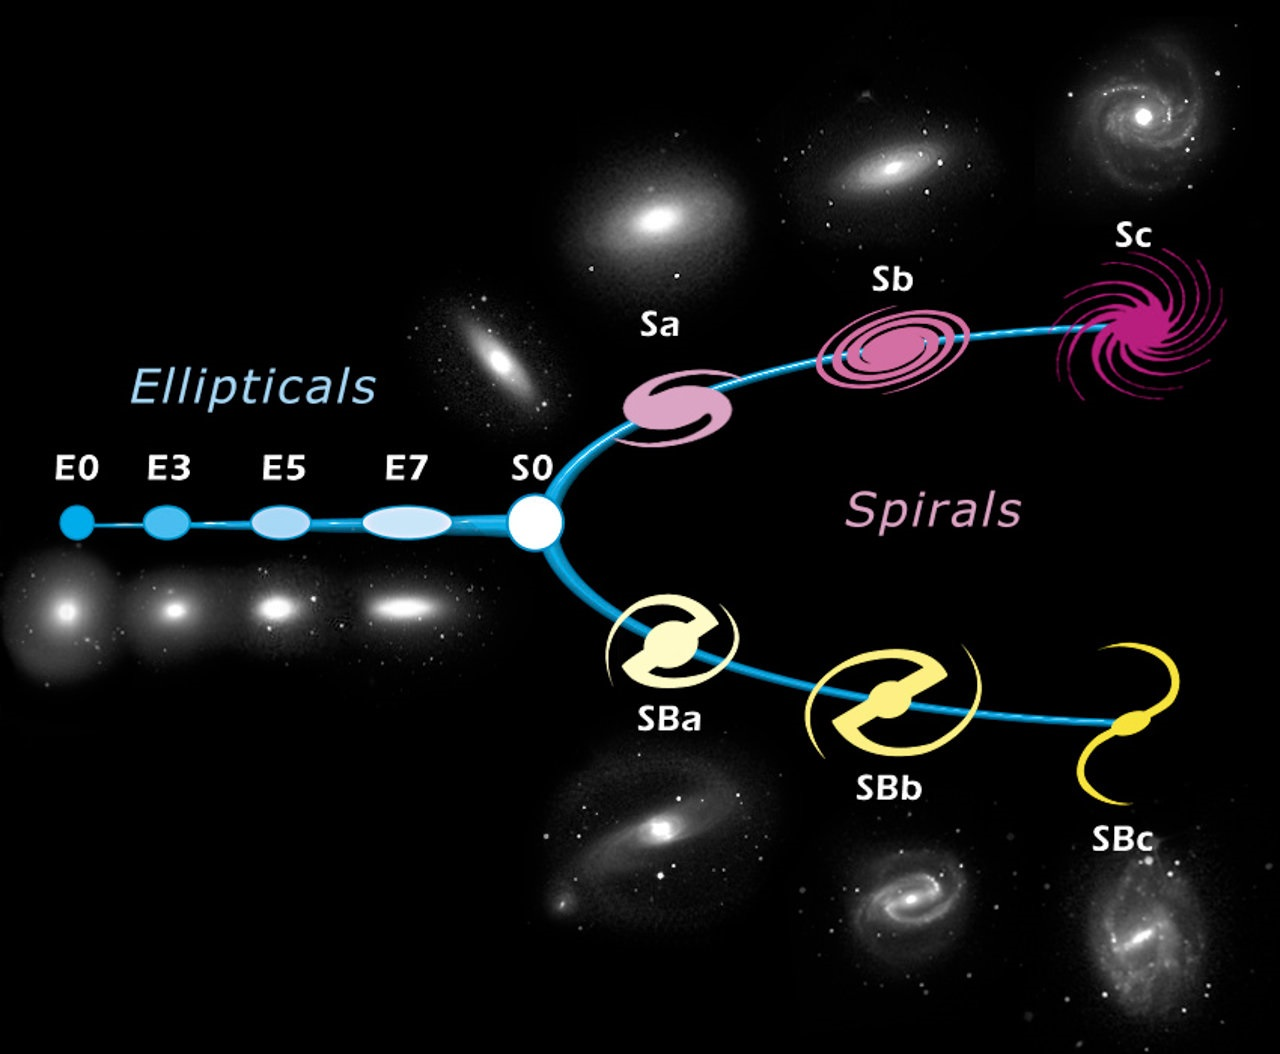
\includegraphics[width=0.6\textwidth]{introduction/hubble.jpg}
		\caption[The Hubble tuning-fork]{Hubble diagram (or tuning fork), showing the different morphology classifications of galaxies. Spirals exist on two sequences: barred and un-barred. The handle of the tuning folk contains ETGs, with S0s being the meeting point of all three sequences. Figure courtesy of http://spacetelescope.org.}
		\label{fig:Hubble}
	\end{figure}

	\begin{figure}
		\centering
		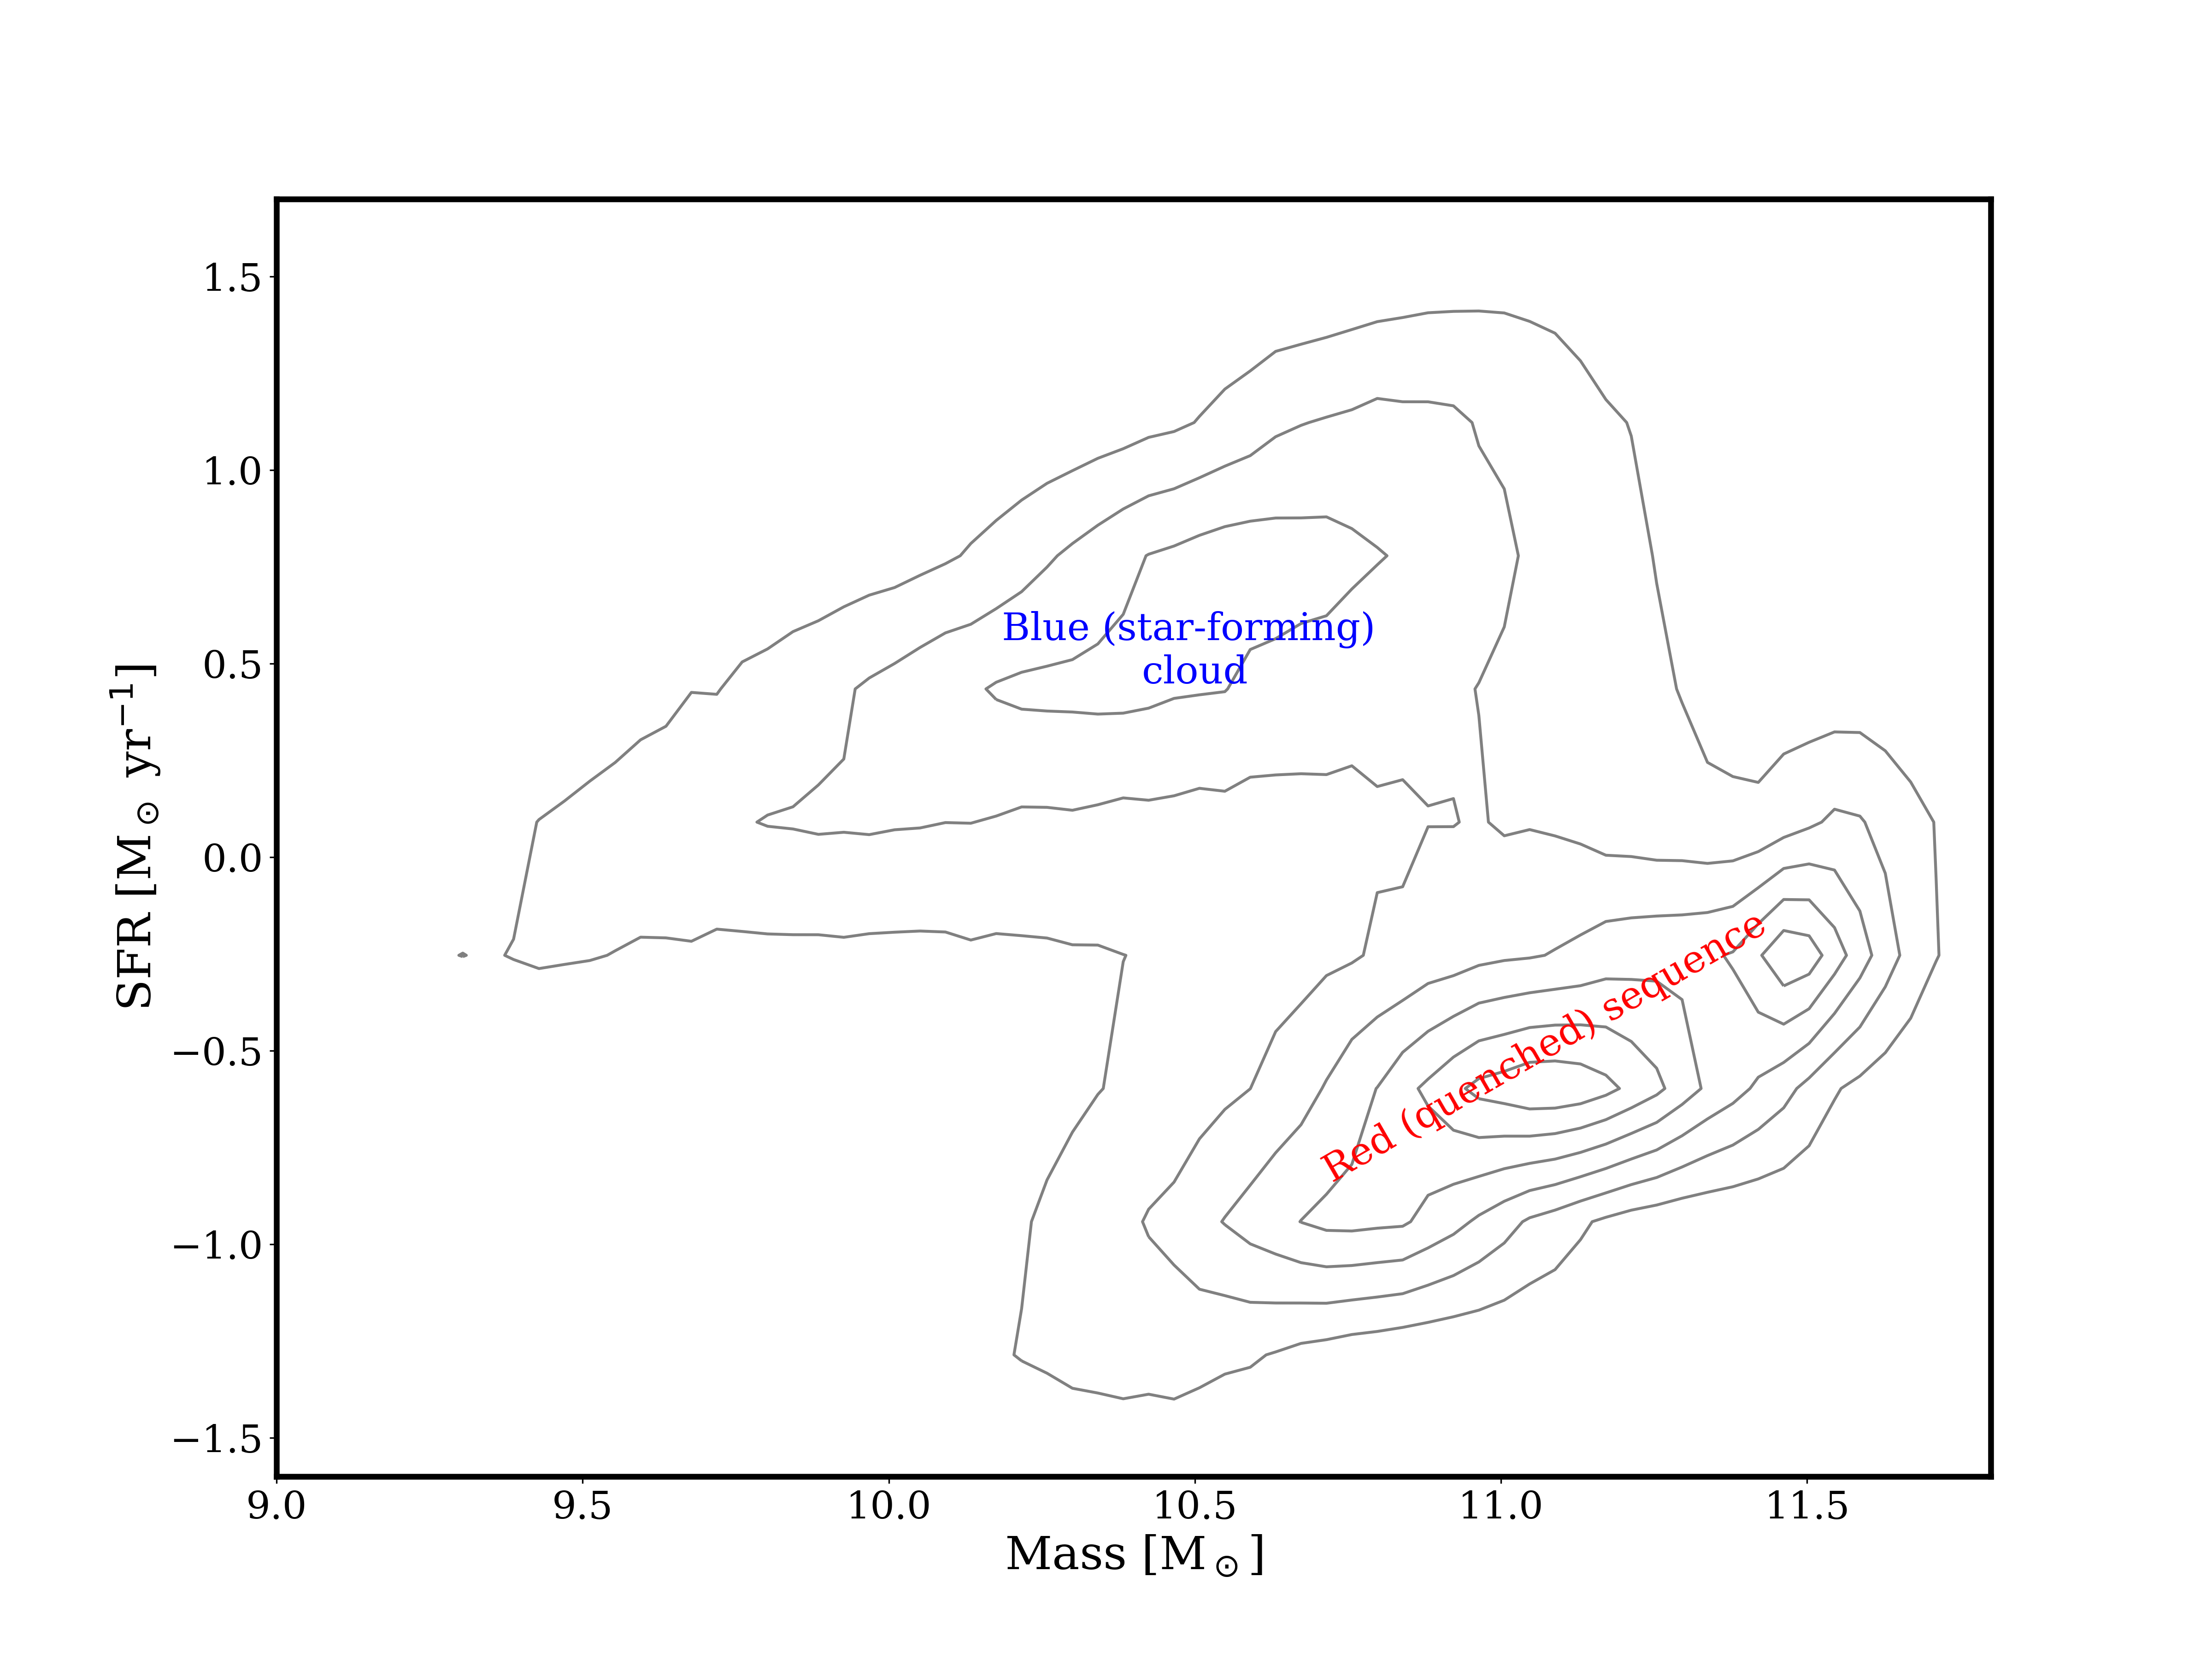
\includegraphics[width=0.7\textwidth]{introduction/sfMass.png}
		\caption[Star-formation rate--galaxy mass diagram]{The star-formation rate--mass plane for the MPA-JHU sample galaxies \citep{Kauffmann2003, Brinchmann2003, Salim2007} clearly showing the dichotomy between the blue cloud and red sequence galaxies.}
		\label{fig:ColourMass}
	\end{figure}

	\begin{figure}
		\centering
		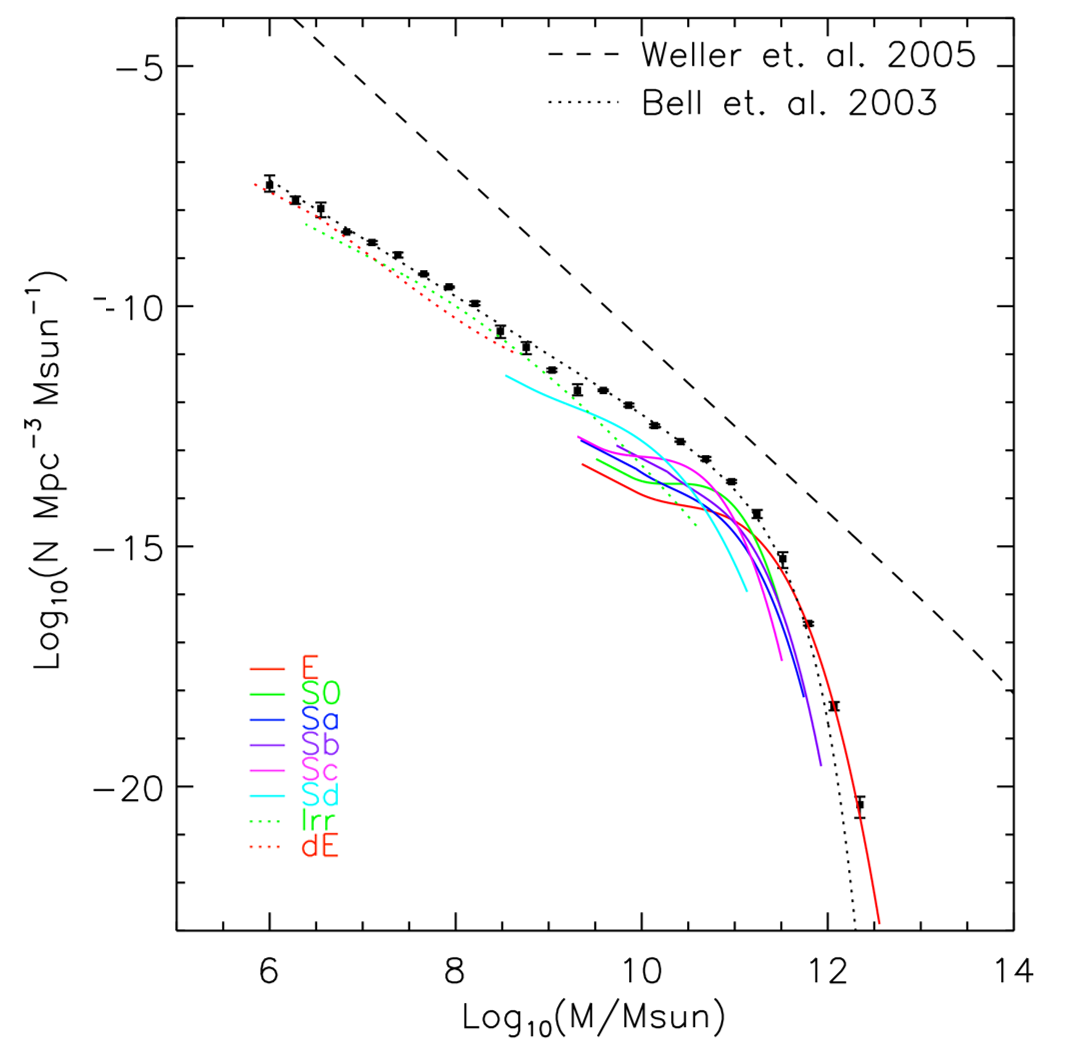
\includegraphics[width=.6\textwidth]{introduction/agnFeedback.png}
		\caption[Galaxy mass function]{Galaxy mass function. The coloured lines (both solid and dotted) show spline fits by Hubble type (ellipticals are shown by the solid red line), while the dashed black line shows the expected dark matter halo mass function \citep{Weller2005} and the dotted line is the Schechter function fit to all galaxies \citep{Bell2003}. Figure courtesy of \citet{Read2005}.}
		\label{fig:massSuppression}
	\end{figure}

	Given their low star formation rates, ETGs are dominated by old stars, while spirals are dominated by young stars. Understanding the reasons for this dichotomy is a major quest of modern astrophysics. ETGs are often the most massive galaxies, so they clearly must have undergone substantial star formation in their early history, that has now stopped. They either must have run out of fuel for forming stars or have experienced (and be experiencing) processes preventing star formation (commonly known as "quenching"). Many have been observed to contain at least some Col.\,(atomic and/or molecular) gas \citep[e.g.][]{Lees1991}, the material from which stars are formed. This seems to favor the latter. The reservoirs are, however, significantly smaller than in LTGs. Without this quenching of star formation, we should expect the galaxy mass function -- number density profile of galaxies shown in Fig.\,\ref{fig:massSuppression} to follow that of dark matter haloes, assuming pure hierarchical growth of overdensities (dashed line in Fig.\,\ref{fig:massSuppression}). Clearly, star-formation is being suppressed at both the high-mass and the low-mass end.

	\begin{figure}
		\centering
		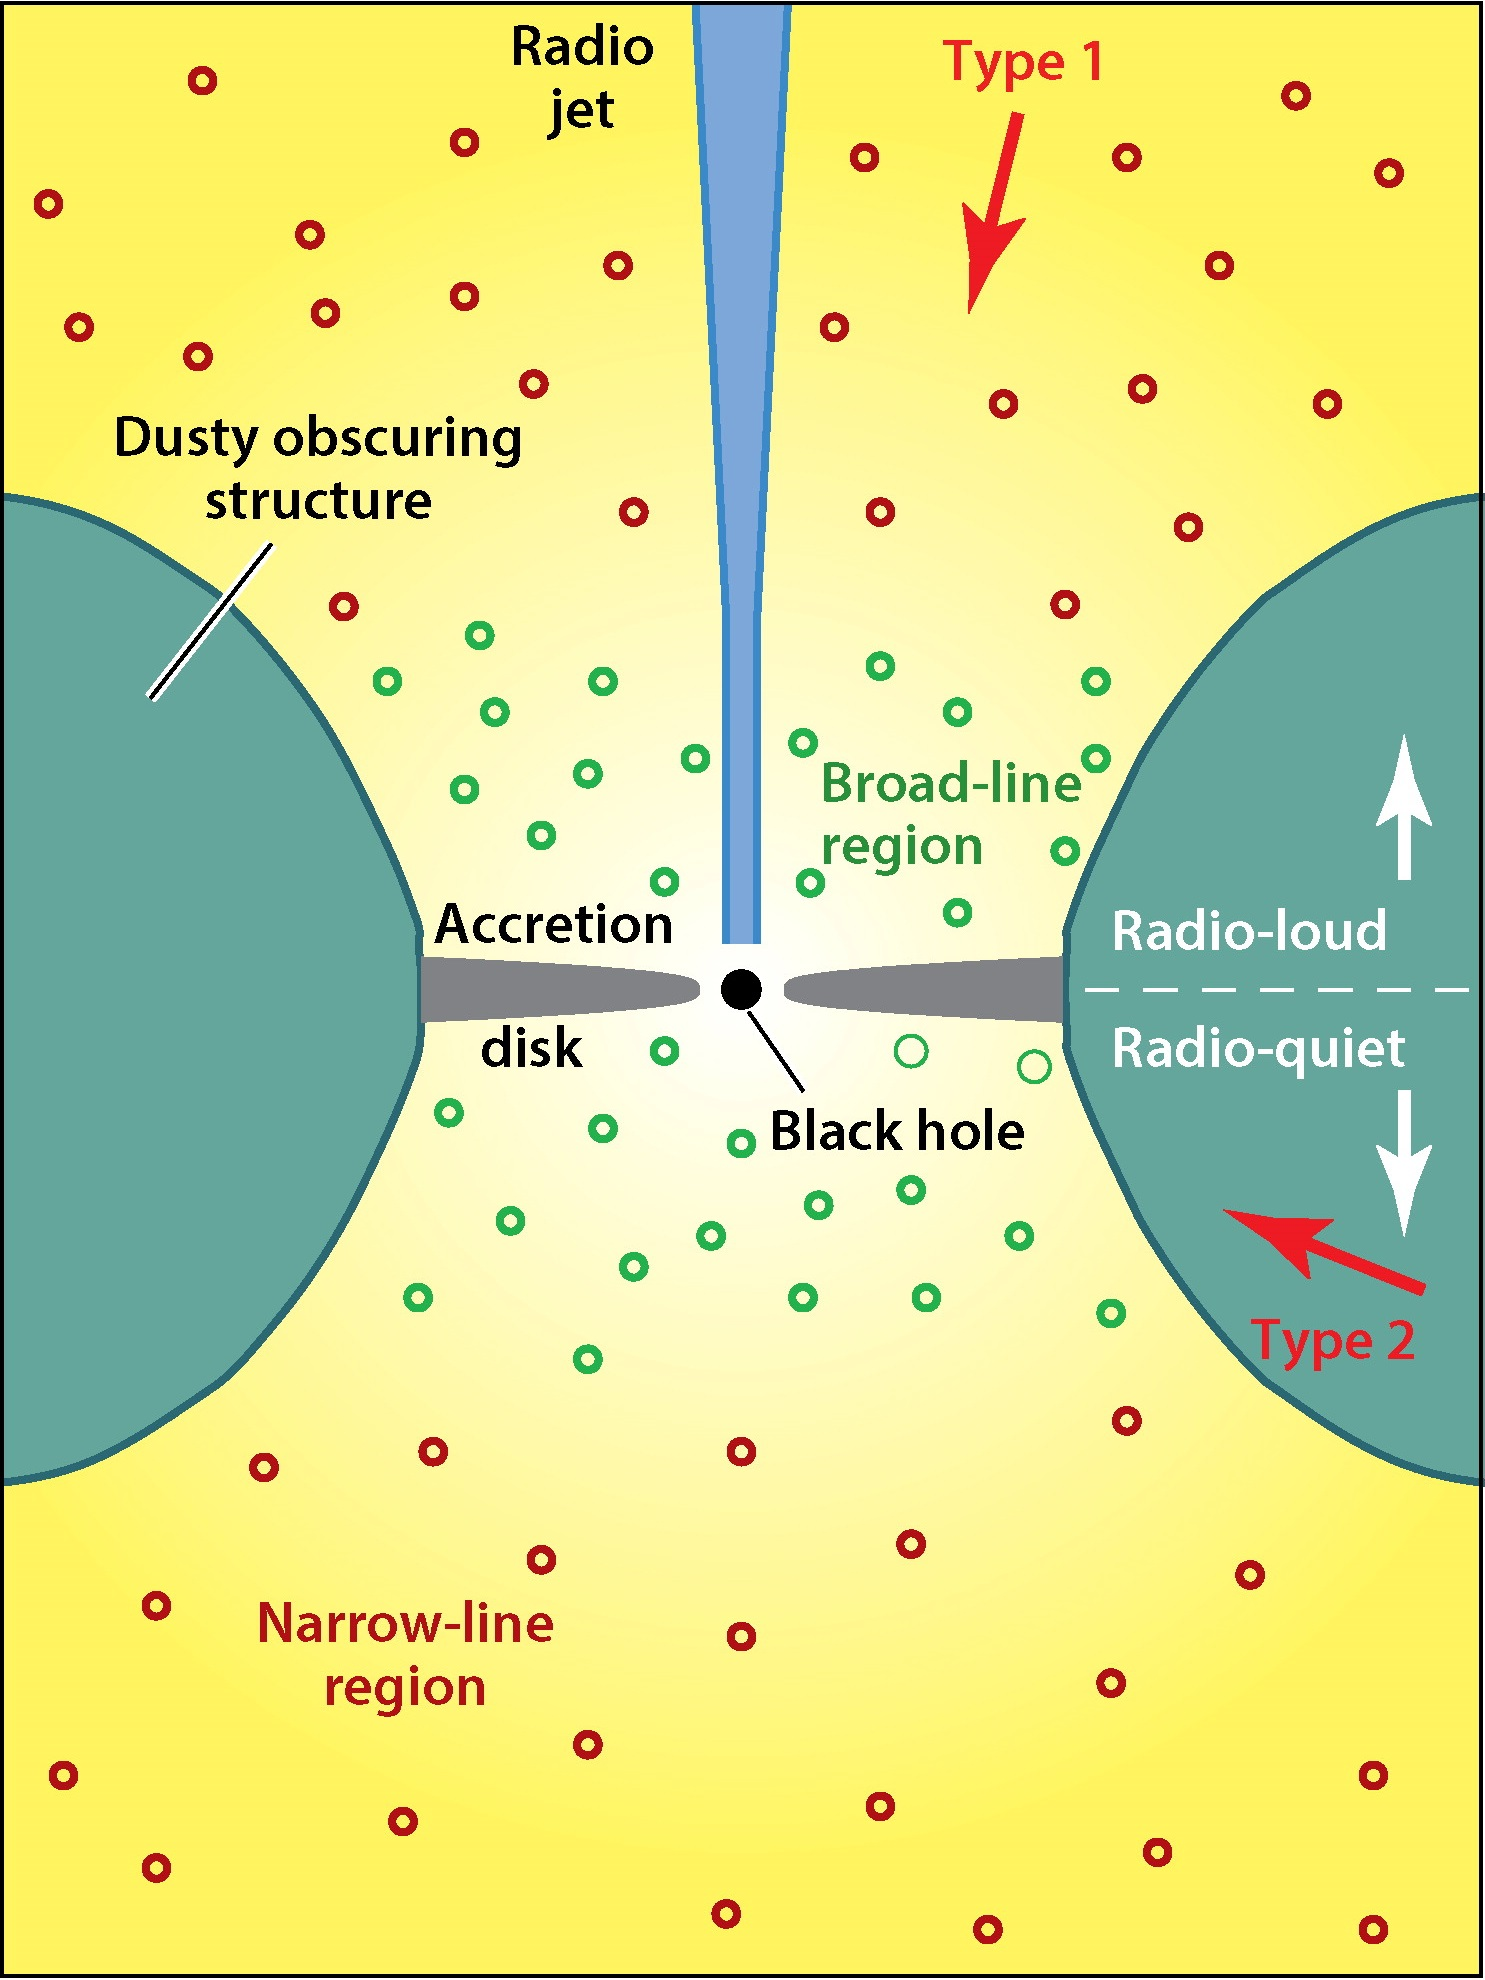
\includegraphics[width=.5\textwidth]{introduction/unifiedAGN.jpeg}
		\caption[Schematic of unified model of AGN]{Schematic of the unified model of AGN. The primary source of radiation is the accretion disc, which in turn ionises both the broad-line and narrow-line regions. A dust torus obscures side-on views (Type 2 AGN), while a jet sometimes emerges from the poles of the disc. Figure courtesy of \citet{Heckman2014}.}
		\label{fig:UnifiedAGN}
	\end{figure}

	Many studies now point to the fact that most (if not all) galaxies contain a super-massive black hole at their centre \citep[e.g.][]{Kormendy2013a}. There are tight correlations (known as scaling relations) between the properties of the central black holes and those of the host galaxies, despite orders of magnitude differences between the spheres of gravitational influence of the black holes and the sizes of the host galaxies \citep[e.g.][]{Gudehus1973, Faber1976, Ferrarese2000, Gebhardt2000}. 

	It is also seen that many galaxies contain a bright point source at their centre. These are known as active galactic nuclei (AGN), and in extreme cases (quasars) they can completely outshine the total starlight of the host galaxy. AGN are understood to be the result of the accretion of  inter-stellar matter (known as the inter-stellar medium; ISM) onto the central black hole \citep[e.g.][]{Lynden-Bell1969}, and the energy released by the AGN is generally invoked to explain the galaxy--black hole scaling relationships \citep[e.g.][]{Raimundo2010} as well as the quenching of star formation in (massive) ETGs \citep[e.g.][]{Croton2006, Somerville2008}. This process is known as AGN feedback and appears to be required by current numerical simulations and semi-analytic models to successfully reproduce the observed properties of massive galaxies \citep[e.g.][]{Kauffmann2000, Granato2004, DiMatteo2005, Springel2005, Bower2006, Croton2006, Hopkins2006, Ciotti2010, Scannapieco2012}. The exact fraction of galaxies that contain an AGN varies depending on the method employed to identify the AGN, but it is strongly mass dependent, with more massive galaxies more likely to contain an AGN \citep[e.g.][]{Kauffmann2003a}.

	AGN are varied, but much work has been done on a single unified model where the differences between individual galaxies can be explained by different orientations of the AGN. The unified model by \citet{Antonucci1993} describes AGN as made up of up to five components or regions surrounding the central black hole. (i) Immediately around the black hole is an accretion disc. Surrounding this is (ii) an obscuring dust torus, blocking side-on views of the black hole and accretion disc. Intense radiation from the accretion disc ionises (iii) the region immediately above and below the disc, which emits in the optical regime. The gas has very high orbital velocities ($\approx 5000 \, \mathrm{km \, s^{-1}}$) due to the proximity to the black hole, giving rise to characteristic broad lines and this region's name: broad-line region (BLR). The BLR is also obscured by the torus if viewed edge-on. Beyond this is (iv) the narrow-line region (NLR), an area of more sedate velocities ($\approx 200 \, \mathrm{km \, s^{-1}}$) and less ionised gas. Because of the shadow cast by the torus, the NLR sometimes appears as conical in shape \citep{Wilson1994}. Finally, a small proportion of AGN contain (v) jets of plasma traveling at relativistic speeds out from the poles of the accretion disc (the exact orientation of the jets may well also be dependent on the orientation of the spins of the black holes, though this remains unknown). The nature of the jets is explored in more detail below. AGN viewed side-on, with the black hole, accretion disc and BLR obscured by the torus are known as Type 2 AGN, while AGN viewed face-on, sometime viewing directly down the jet, are known as Type 1. A schematic of the unified model is shown in Fig.\,\ref{fig:UnifiedAGN}.


	Despite the unification of the many observed morphologies of AGN, it is becoming increasingly clear that AGN exist in two different modes, radiative and jet mode \citep[e.g.][]{Antonucci2012}, raising speculation about differing mechanisms and possibly fuel sources for each. More detail on both modes can be found in Section \ref{sec:AGN}. 


	Most galaxies also emit at radio frequencies. These galaxies are known as radio galaxies (RGs). Mostly this is attributed to star formation, which radiates due to free-free (thermal) emission from regions of ionised ISM (\ion{H}{ii} regions) and synchrotron emission from supernova remnants as relativistic electrons spiral along the strong magnetic field lines. Except in extreme star bursts, radio emission due to star formation is fairly low-level. Many AGN also emit in at radio frequencies due to synchrotron emission from the jets. Not considering star bursts, the brightest sources can be considered bona-fide detections of the AGN jets. However, distinguishing between star-formation and AGN jets can be difficult for fainter sources, though there is no consensus on where this transition should lie. Emission from AGN will always be from the centre of the galaxy (the location of the AGN) and extending out along the trajectory of the jets. However, \citet{Nyland2016} note that in the fainter centrally concentrated RGs, the radio emission is also consistent with circumnuclear star formation.

	There is broad consensus within the literature that the most powerful RGs ($\log P_\mathrm{1.4\, GHz}/(\mathrm{W \, Hz^{-1}}) \gtrsim 25.5$) are the product of gas-rich (wet) major mergers of galaxies (a major merger is defined as a merger of galaxies with a mass ratio smaller than 3:1). These AGN tend to be extremely luminous. Indeed, despite clearly containing a very powerful jet, they are mostly radiative mode AGN. These RGs form a very small minority of the RG population and hence are not representative. Indeed, \citet{Heckman2014} present evidence that most RGs are fueled through secular processes.

	This thesis will compare and contrast the stellar and ionised gas properties of RGs and radio-quiet ETGs. The rest of this chapter will thus cover the background required to study the RG population. Firstly, since RGs are primarily found in ETGs, the current understanding of ETGs will be reviewed. This is mostly a summary of the recent integral field spectroscopy (IFS) surveys including Atlas$^\text{3D}$, MaNGA, MASSIVE, SAMI and Califa, and can be considered as setting out of the control sample for later investigations (see Section \ref{sec:ETG}). Secondly, in Section \ref{sec:AGN}, a more detailed summary of the current state of our understanding of AGN will be presented, including RGs. Finally, the selection criteria of the sample used throughout this thesis will be described (Section \ref{sec:Sample}).

	Chapter \ref{cha:Data} gives details of the VIMOS and MUSE instruments, as well as the corresponding data reduction and analysis methods. Chapters \ref{cha:stellar} and \ref{cha:gas} cover the results, focusing on the stellar and ionised gas components, respectively, of the sample galaxies. Chapter \ref{cha:conclusion} presents a summary and conclusions. 

\section{Early-type Galaxies}
	\label{sec:ETG}
	Confusingly, due to historical reasons, there are several similar yet subtly different definitions of the LTG/ETG classes. Originally they were based purely on the morphology as seen in optical images: spirals were LTGs and ellipticals were ETGs, while there was debate about which class lenticular galaxies (S0s) belonged to. S0s appear disc-like like LTGs, but often contain older populations with less star formation like ETGs. This debate has confused the literature, with some taking the classification scheme to reflect the underlying stellar population and others the assumed method of dynamical support (rotation vs dispersion). In this thesis we use the stellar population view and as such include S0s within the ETG class.

	A useful morphological sub-classification within ETGs is the slope of the nuclear surface brightness profile. Some galaxies show a significant flattening of their surface brightness profile towards the centre of the galaxy (cored galaxies), whereas others show only a mild change (power-law galaxies). An example of each class is shown in Fig.\,\ref{fig:CorePower}. This is parametrised using a double power-law of the form
	\begin{align}
		\Sigma(R) = & \, \Sigma_\mathrm{b} \left(\frac{R_\mathrm{b}}{R}\right)^\gamma \left[\frac{1}{2} + \frac{1}{2}\left(\frac{R}{R_\mathrm{b}}\right)^\alpha\right]^{\frac{\gamma-\beta}{\alpha}} \, ,
		\label{eq:Nuker} \\
		\intertext{where $\gamma$ and $\beta$ control the inner and outer slope, respectively, $R_\mathrm{b}$ is the radius of the transition between the inner and out slopes, $\Sigma_\mathrm{b}$ is the surface brightness at $R_\mathrm{b}$ and $\alpha$ sets the speed of the transition. A galaxy is classifed using the derivative $\gamma'$:}
		\gamma' \equiv & \, - \left. \frac{\mathrm{d}\log I}{\mathrm{d} \log R} \right|_{R=R'} = - \frac{\gamma + \beta \left(\frac{R'}{R_\mathrm{b}}\right)^\alpha}{1 + \left(\frac{R'}{R_\mathrm{b}}\right)^\alpha}
	\end{align}
	evaluated at \textit{Hubble Space Telescope's (HST)} resolution limit of $R' = 0.1"$. A galaxy with $\gamma' \le 0.3$ is a considered a cored galaxy, while one with $\gamma' \ge 0.5$ is called a power-law (or `cuspy') galaxy. In the range $0.3 < \gamma' < 0.5$, galaxies are considered intermediate. High-resolution images have shown that cored galaxies typically have `boxy' isophotes, while power-law galaxies typically have `discy' isophotes \citep[e.g.][]{Lauer1995, Faber1997}. In addition, these are respectively thought to correspond to triaxial and oblate 3 dimensional shapes \citep[e.g.][]{Krajnovic2011, Krajnovic2013a, Krajnovic2013}.

	\begin{figure}
		\centering
		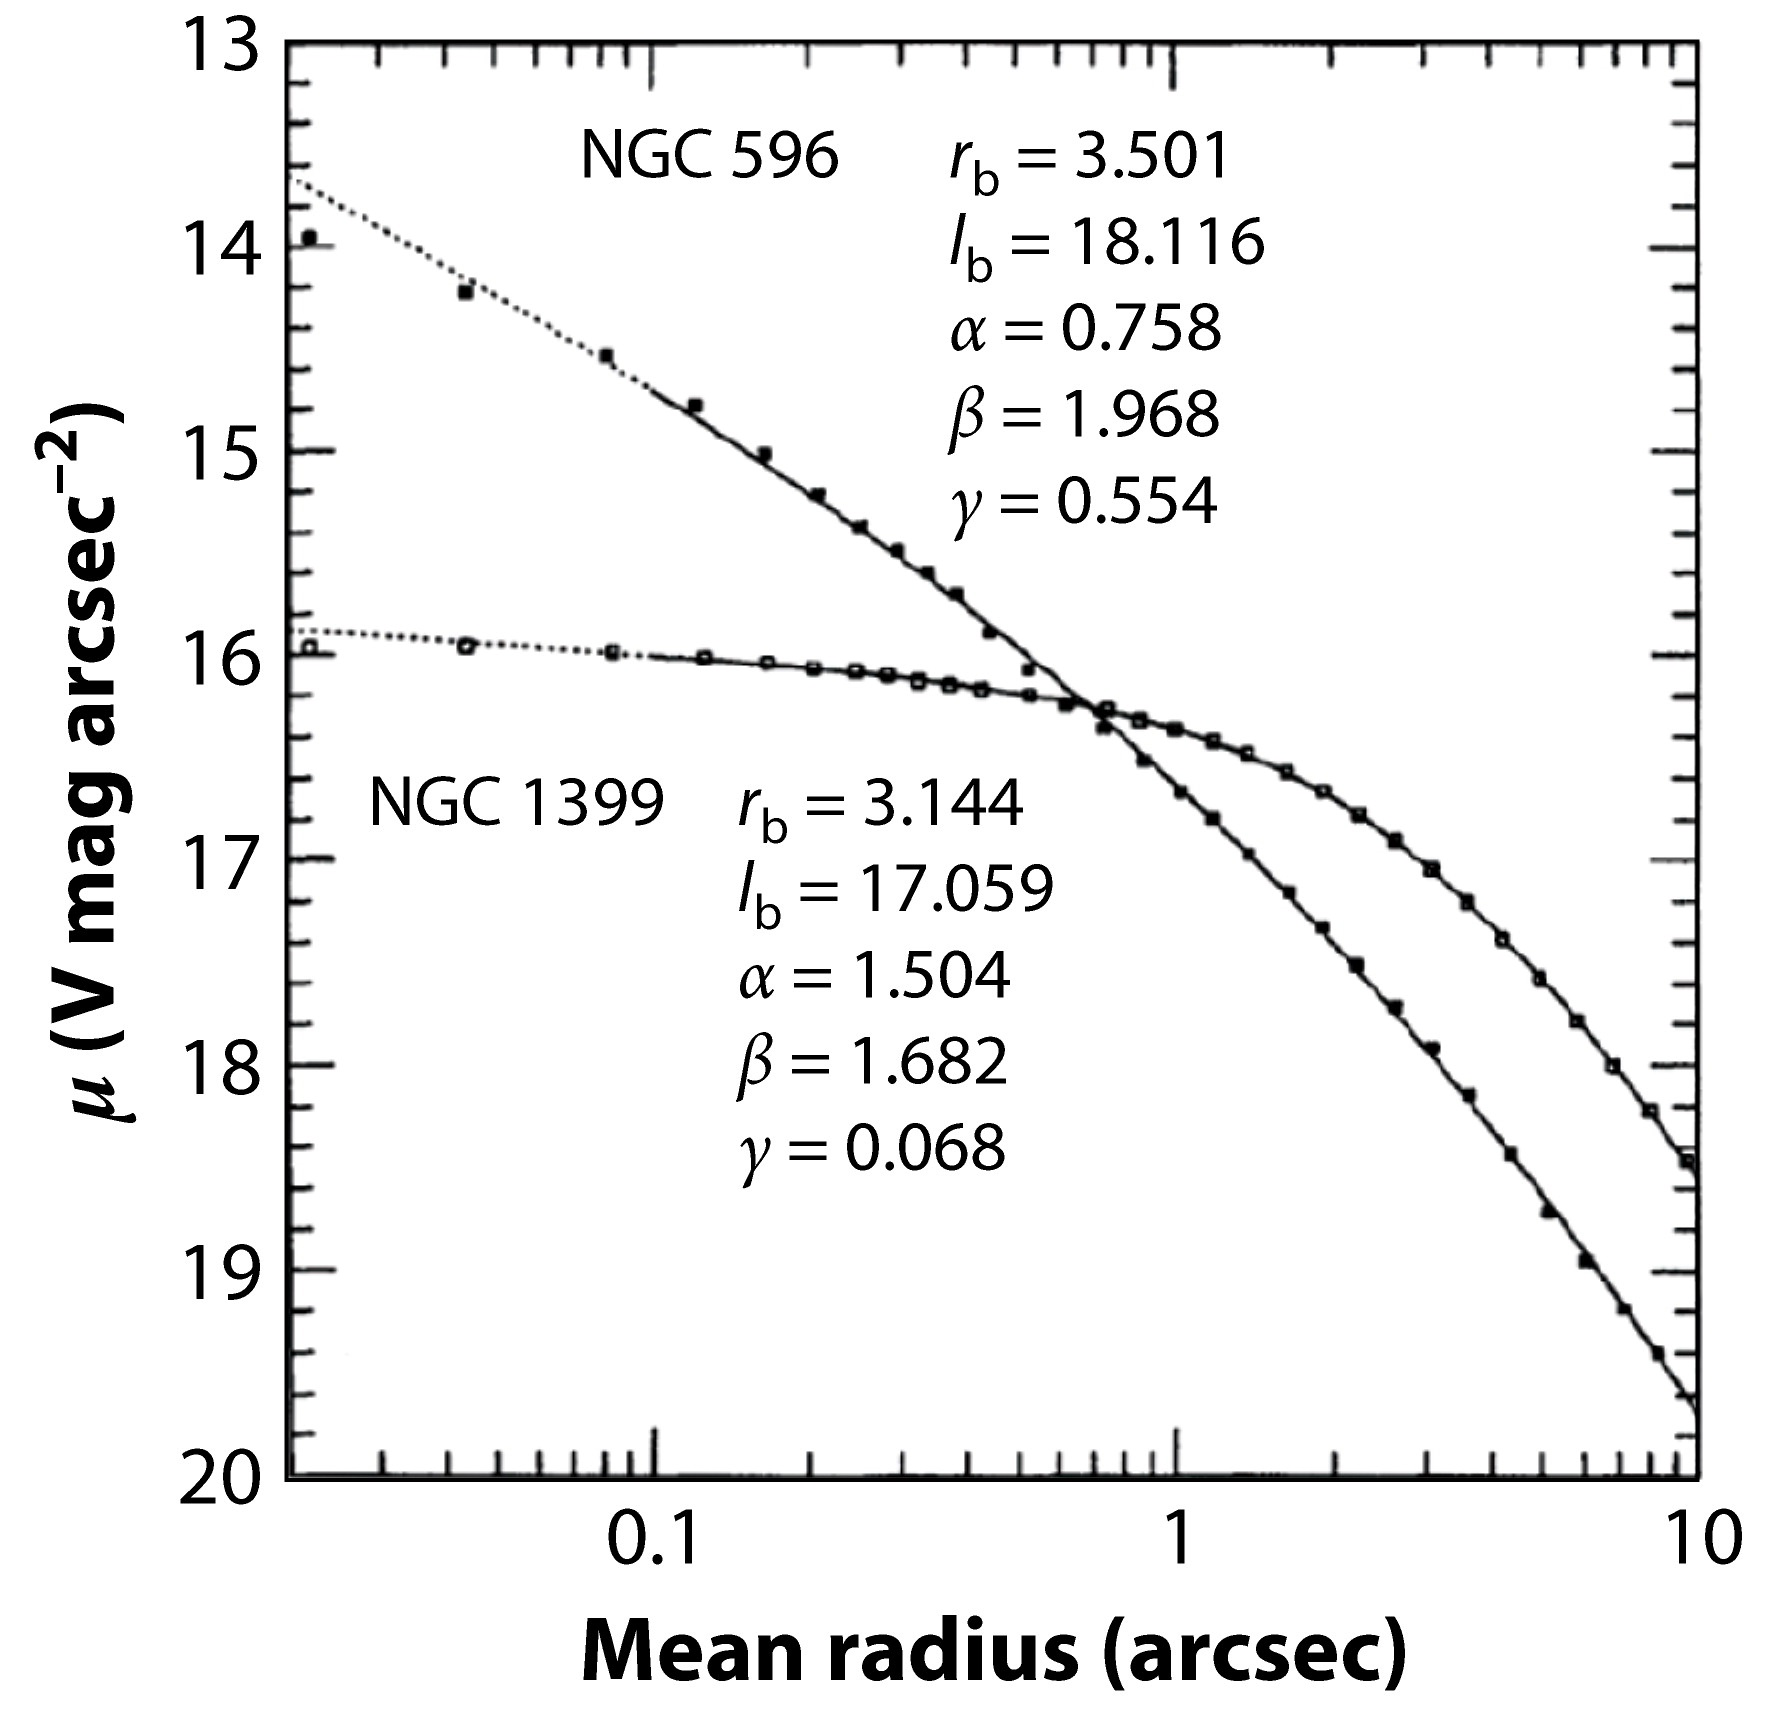
\includegraphics[width=0.5\textwidth]{introduction/exampleCorePower.jpeg}
		\caption[Example of cored and power-law surface brightness profile]{Examples of power-law (NGC 596) and cored (NGC 1399) surface brightness profiles. Both are fit with a double power law (Eq. \ref{eq:Nuker}), shown with the black lines. Both galaxies have similar outer slopes but dramatically different inner slopes. Figure courtesy of \citet{Lauer1995}.}
		\label{fig:CorePower}
	\end{figure}

	The Atlas$^\text{3D}$ survey \citep{Cappellari2011} found that morphologically categorising ETGs into ellipticals and S0s is misleading and does not not reflect any underlying physical difference. Instead it used spatially-resolved stellar kinematics to classify ETGs into fast or slow rotators, depending on their value of $\lambda_R$ \citep{Emsellem2011}, where $\lambda_R$ is a parameter that quantifies a galaxy's specific angular momentum and is defined as
	\begin{align}
		\lambda_R \equiv & \frac{\langle R |V|\rangle}{\langle R \sqrt{V^2 + \sigma^2}\rangle} \, ,\\
		\intertext{where the angled brackets represent flux-weighted averages within a radius $R$, $V$ is the mean stellar velocity and $\sigma$ is the stellar velocity dispersion. For spatially-binned data:}
		\lambda_R = & \frac{\sum_{i=1}^{N} F_i R_i |V_i|}{\sum_{i=1}^{N} F_i R_i \sqrt{V_i^2 + \sigma_i^2}} \, ,
	\end{align}
	where $F_i$ is the flux of the $i^\text{th}$ bin, $R_i$ its distance from the centre and $V_i$ and $\sigma_i$ its mean stellar velocity and velocity dispersion, respectively. The sum is computed over all $N$ bins with a radius $R$. 

	The most recent definition of a slow rotator is
	\begin{equation}
		\lambda_\mathrm{R_e} < 0.08 + \frac{\epsilon}{4} \text{    and    } \epsilon < 0.4 \, ,
	\end{equation}
	where $\epsilon$ is the galaxy ellipticity and $\lambda_\mathrm{R_e}$ the value of $\lambda_R$ evaluated at the effective radius $\mathrm{R_e}$ \citep{Cappellari2016}. % Need to find original place this was defined (not just Michele's review).
	It is worth noting here that while most S0s are fast rotators and most slow rotators are ellipticals, the converses are not necessarily true: many ellipticals are fast rotators and some slow rotators are S0s. In fact the dichotomy is better reflected by the cored verse power-law morphologies, though \citet{Cappellari2016} notes that the kinematic classification scheme has the advantage that it is nearly inclination independent and can be measured at much lower spatial resolution. Having said that, the cases where the two classifications do not agree are often due to misclassified kinematics, such as counter-rotating stellar discs erroneously classified as slow rotators \citep[e.g.][]{Pinkney2003, Cappellari2005, Cappellari2007}. 

	Most slow rotators are massive, with stellar masses $M_\ast \gtrsim 10^{10.5} M_\odot$ and they dominate the high-mass end of the galaxy mass function, though fast rotators dominate in number by a factor of $\approx 7$ \citep[e.g.][]{Emsellem2011, Veale2017}. Fig.\,\ref{fig:SlowRotFrac} shows the change in the proportion of slow rotators as a function of stellar mass (for which $K$-band magnitude, $M_K$, is used as a proxy).


	\begin{figure}
		\centering
		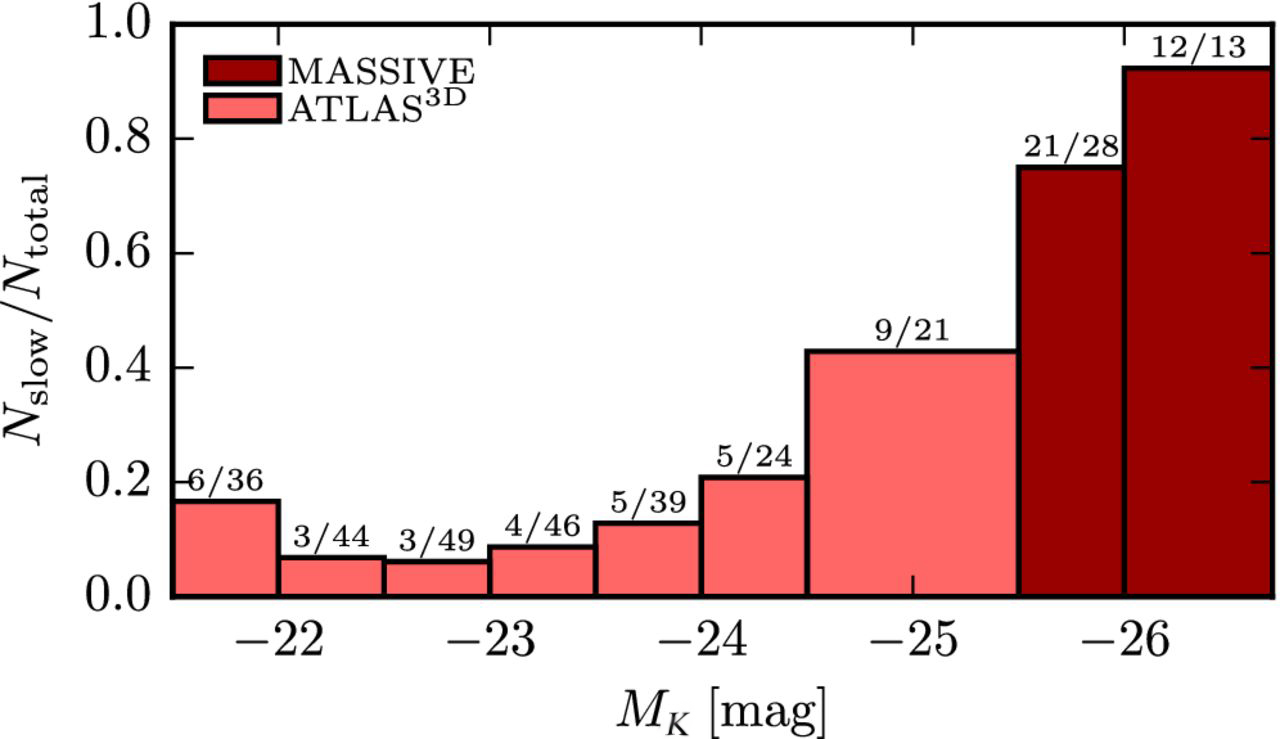
\includegraphics[width=0.8\textwidth]{introduction/slowRotFraction.jpeg}
		\caption[Proportion of slow rotating galaxies as a function of mass]{The fraction of slow rotators (within the total number of galaxies) as a function of total $K$-band magnitude ($M_K$), used as a proxy for total stellar mass. Figure courtesy of \citet{Veale2017}.}
		\label{fig:SlowRotFrac}
	\end{figure}

	Fast rotators reflect many properties of and have strikingly similar spatial distributions to spirals. Fast rotators have been shown to contain discs, and even very round objects can be shown to be face-on discs \citep[e.g.][]{Cappellari2013a, Weijmans2014}. They also have very similar bulge-to-disc ratios to spirals \citep{Krajnovic2013}. In Fig.\,\ref{fig:MassRe}, fast rotators form a parallel sequence to spiral galaxies.

	The discovery of the fast/slow-rotator scheme re-ignites the S0 debate and led the Atlas$^\text{3D}$ team to re-evaluate the Hubble sequence. In its place they proposed the Atlas$^\text{3D}$ comb (shown in Fig.\,\ref{fig:Atlas3Dcomb}; \citealt{Cappellari2011a}) where fast rotating ETGs form a parallel sequence to spirals in the scaling relationship (e.g. the galaxy mass--size plane; see Fig.\,\ref{fig:MassRe}), but share many properties such as stellar age and gas content with slow rotating ETGs. 

	\begin{figure}
		\centering
		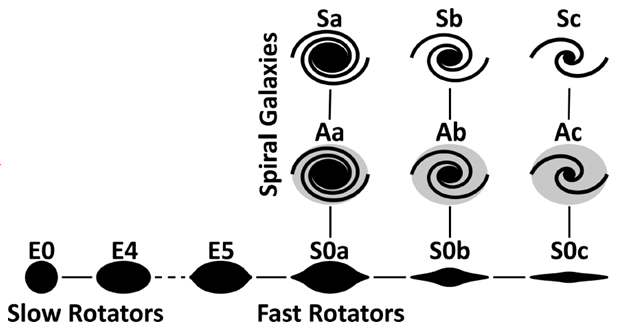
\includegraphics[width=0.8\textwidth]{introduction/Atlas3D_comb.png}
		\caption[The Atlas$^\text{3D}$ comb]{The Atlas$^\text{3D}$ comb, a replacement of the Hubble tuning fork (Fig.\,\ref{fig:Hubble}). ETGs (bottom row) form a parallel sequence to spirals in terms of the rotation and bulge-to-disc ratio. Solid lines show empirical continuity, while the dashed line represents the discontinuity between the fast and slow rotators. The intermediate `anemic' spirals, as classified by \citet{VandenBergh1976}, are included to demonstrate the continuous nature of the link between S0s and spirals. Figure courtesy of \citet{Cappellari2011a}.}
		\label{fig:Atlas3Dcomb}
	\end{figure}

	Since \citet{Sarzi2015} showed inner power-laws against be fragile to dry major mergers, cores are assumed to be markers that the galaxy has undergone such a merger. The near 1:1 correspondence between the slow/fast rotators and cored/power-law classifications shows that dry major mergers must also be responsible for forming slow rotators and changing the shapes of galaxies from oblate to triaxial.

	One useful test for a triaxial shape is misalignment between the kinematic (rotation) axis and the apparent morphological minor axis. For oblate structures, the two should align within $\approx 5\degree$, but for triaxial structures they can have any misalignment \citep[e.g.][]{Contopoulos1956, Stark1977, Statler1987}. This is seen in Fig.\,\ref{fig:Misalignment}, where regular rotators have aligned photometric and kinematic position angles, and non-regular rotators have any value for the misalignment and low ellipticities. This supports the argument for fast rotators to be axisymmetric oblates, while slow rotators are triaxial, but fairly spherical.

	\begin{figure}
		\centering
		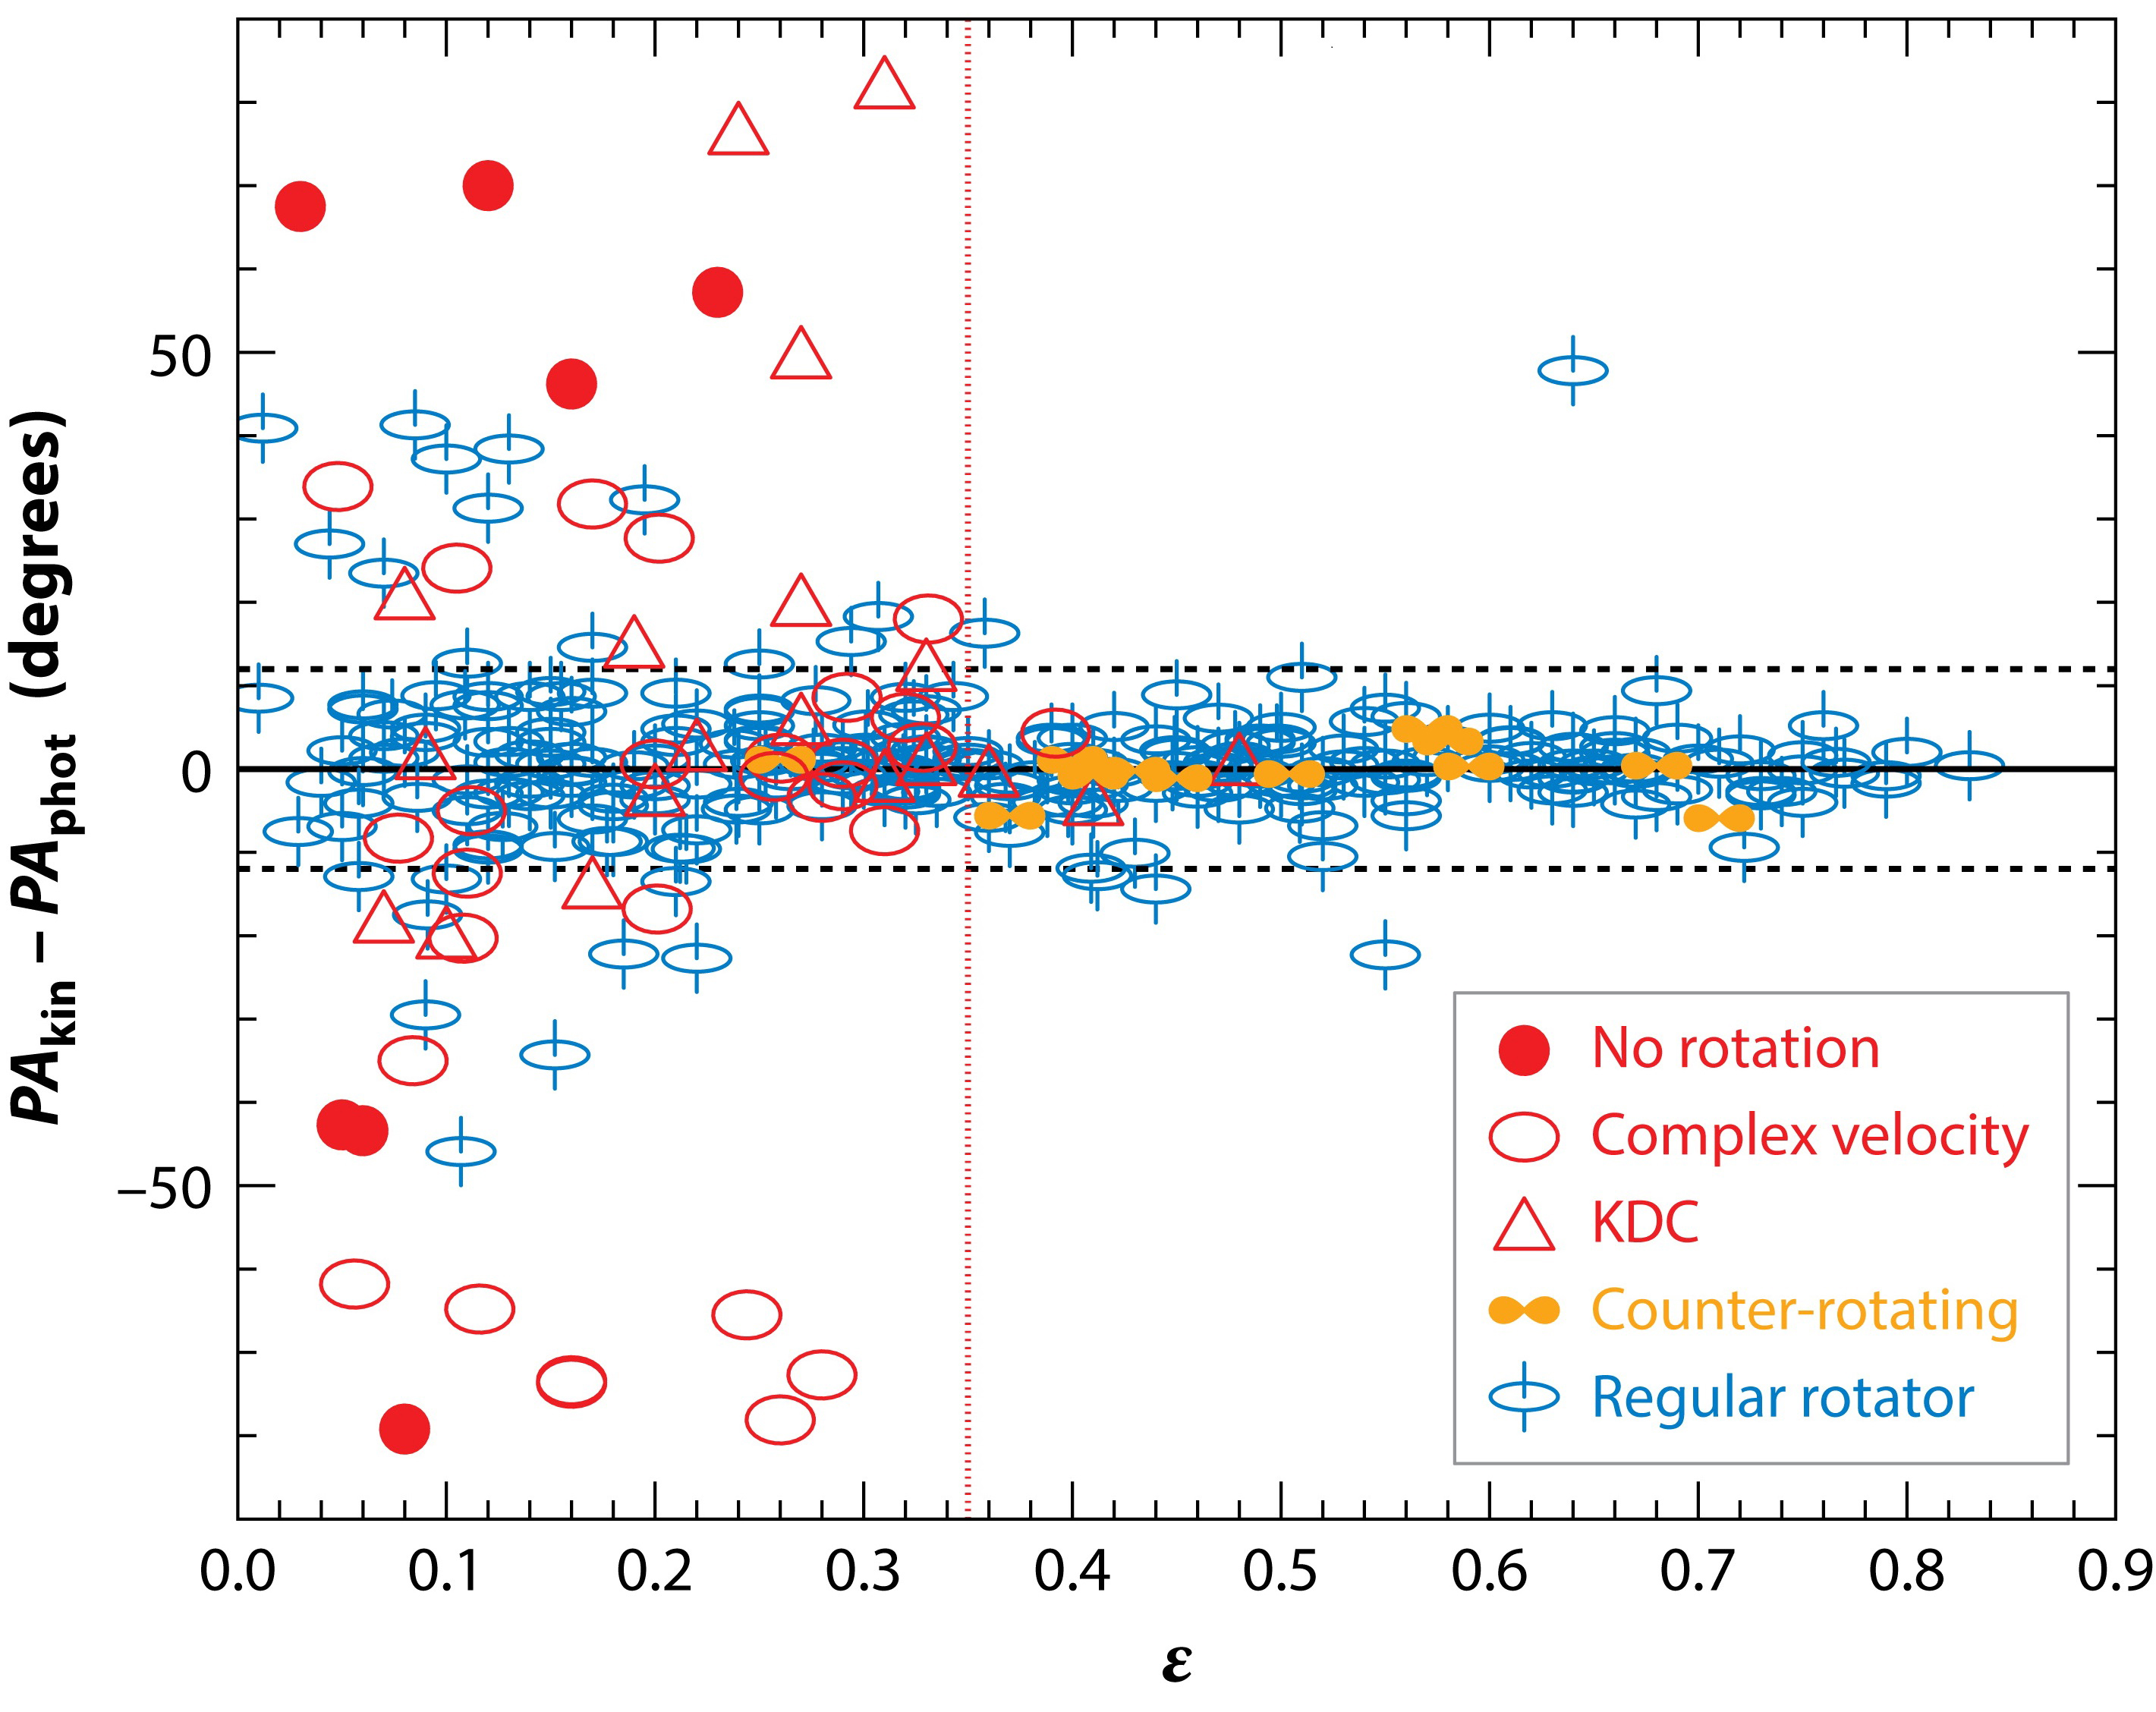
\includegraphics[width=0.7\textwidth]{introduction/misalignment.jpg}
		\caption[The kinematic--photometric misalignment in slow rotators]{Misalignment of the position angles (PAs) of galaxies in the Atlas$^\text{3D}$ and SAMI pilot surveys. Figure courtesy of \citet{Cappellari2016}. KDC is the abbreviation of kinematically decoupled cores.}
		\label{fig:Misalignment}
	\end{figure}

	Fig.\,\ref{fig:MassRe} shows the parallel sequence of S0s to spiral galaxies represented in the Atlas$^\text{3D}$ comb on the galaxy mass--size plane. Galaxies are thought to evolve by gas accretion maintaining roughly constant radii. This increases the bulge-to-mass ratio, moving accreting galaxies from right to left along the fast rotator/spiral section of the Atlas$^\text{3D}$ comb. Major dry mergers transform the galaxies into slow rotators \citep[e.g.][]{Bendo2000} with similar properties to those observed by Atlas$^\text{3D}$ \citep[e.g.][]{Jesseit2007, Jesseit2009}. After this, galaxies increase in mass due to continuous minor mergers \citep[e.g.][]{DeLucia2007, Genel2008, Feldmann2010, Oser2010, Feldmann2011, Hirschmann2012}. This moves the galaxy from the lower-centre to the upper-right of Fig.\,\ref{fig:MassRe}. 

	\begin{figure}
		\centering
		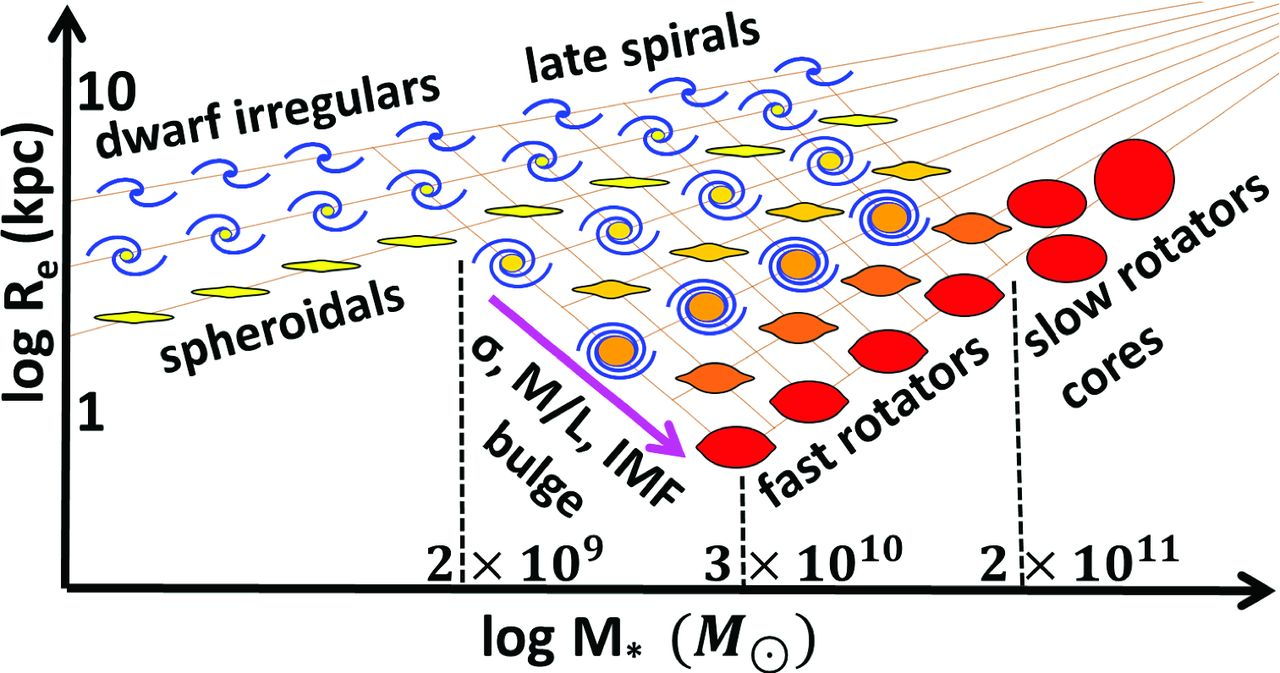
\includegraphics[width=0.7\textwidth]{introduction/mass_Re.jpg}
		\caption[The galaxy mass--size plane]{Galaxy mass--size plane, clearly showing the parallel sequences of S0s and spirals represented by in Atlas$^\text{3D}$ comb. Figure courtesy of \citet{Cappellari2013a}.}
		\label{fig:MassRe}
	\end{figure}

	Atlas$^\text{3D}$ also found a raft of kinematic substructures or features. These were split into five categories, a-e (examples shown in Fig.\,\ref{fig:EgSubstructure}), with a sixth category, f, containing unclassifiable objects \citep{Krajnovic2011}. These are mostly based on the results from the \textsc{kinemetry} routine\footnote{http://davor.krajnovic.org/idl/}\citep{Krajnovic2006}, which parametrises the stellar velocity map with a Fourier decomposition. The best-fitting ellipse is determined by minimizing all Fourier coefficients up the 3rd coefficient, $k_3$, except for the cosine term. Deviations from the cosine law are then represented by the $k_5$ harmonic \citep{Krajnovic2006}. Regular rotators (RRs; or galaxies that are well described by the cosine law) are defined as $\langle k_5/k_1 \rangle < 0.04$, which is based on the mean uncertainty of $k_5/k_1$ of $\approx 0.03$ for all Atlas$^\text{3D}$ galaxies. All other galaxies are classed as non-regular rotators (NRRs). While the RR/NRR classifications broadly reflect the fast/slow rotator classification, they should not be taken to have the same meaning. 

	Various kinematic features were also observed across the Atlas$^\text{3D}$ sample \citep{Krajnovic2011}. Galaxies are flagged as having
	\begin{itemize}
		\item \textbf{No feature (NF)}, if the position angle of the best-fit ellipse, $PA_\mathrm{kin}$, is constant with radius.
		\item \textbf{Double maxima (2M)}, if the radial profile of $k_1$ rises to a local maximum followed by a fall and another subsequent rise. The outer maximum is usually larger than the inner one. 
		\item \textbf{Kinematic twist (KT)}, if $PA_\mathrm{kin}$ varies smoothly with an amplitude of at least 10$\degree$. 
		\item \textbf{Kinematically decoupled/distinct core (KDC)}, if there is an abrupt change of $PA_\mathrm{kin}$ by more than 30$\degree$ and $k_1$ drops to near zero in the transition region. \textbf{Counter-rotating cores (CRCs)} are a special case where the change of $PA_\mathrm{kin}$ is about 180$\degree$.
		\item \textbf{Low velocities (VL)}, if $k_1 < 5 \, \mathrm{km \, s^{-1}}$, below the threshold of \textsc{kinemetry} to establish the ellipse parameters. These galaxies can be considered as non-rotating.
		\item \textbf{Double $\mathrm{\sigma}$ (2$\mathrm{\sigma}$)}, if there are two off-centre but symmetric peaks in the stellar velocity dispersion. These galaxies are understood to contain two counter-rotating discs. 
	\end{itemize}
	Examples of each of the features above can be seen in Fig.\,1 of \citet{Krajnovic2011}. The matching of these features with substructure categories is given in Table \ref{tab:KinGroups}, which also lists the total number of galaxies in each category in the Atlas$^\text{3D}$ sample. 

	\begin{table}
		\centering
	\begin{threeparttable}
		\caption{Kinematic groups defined by Atlas$^\text{3D}$.}
		\label{tab:KinGroups}
		\begin{tabular}{c l l}
			\hline
			\hline
			Group 	& N$_\text{gals}$ & Features \\
			\hline
			a 		& 7			& NRR/LV \\
			b 		& 12		& NRR/NF \\
			c 		& 19		& NRR/KDC, NRR/CRC, RR/CRC \\
			d 		& 11		& NRR/2$\mathrm{\sigma}$, RR/2$\mathrm{\sigma}$ \\
			e 		& 209		& RR/NF, RR/2M, RR/KT \\
			f 		& 2			& Unclassified \\
			\hline
			\hline
		\end{tabular}
		\begin{tablenotes}
		\footnotesize
		\note Col.\,1: Kinematic group. Col.\,2: number of galaxies from the Atlas$^\text{3D}$ sample out of 260. Col.\,3: kinematic features defining the group. Table reproduced from \citet{Krajnovic2011}.
		\end{tablenotes}
	\end{threeparttable}
	\end{table}

	\begin{figure}
		\centering
		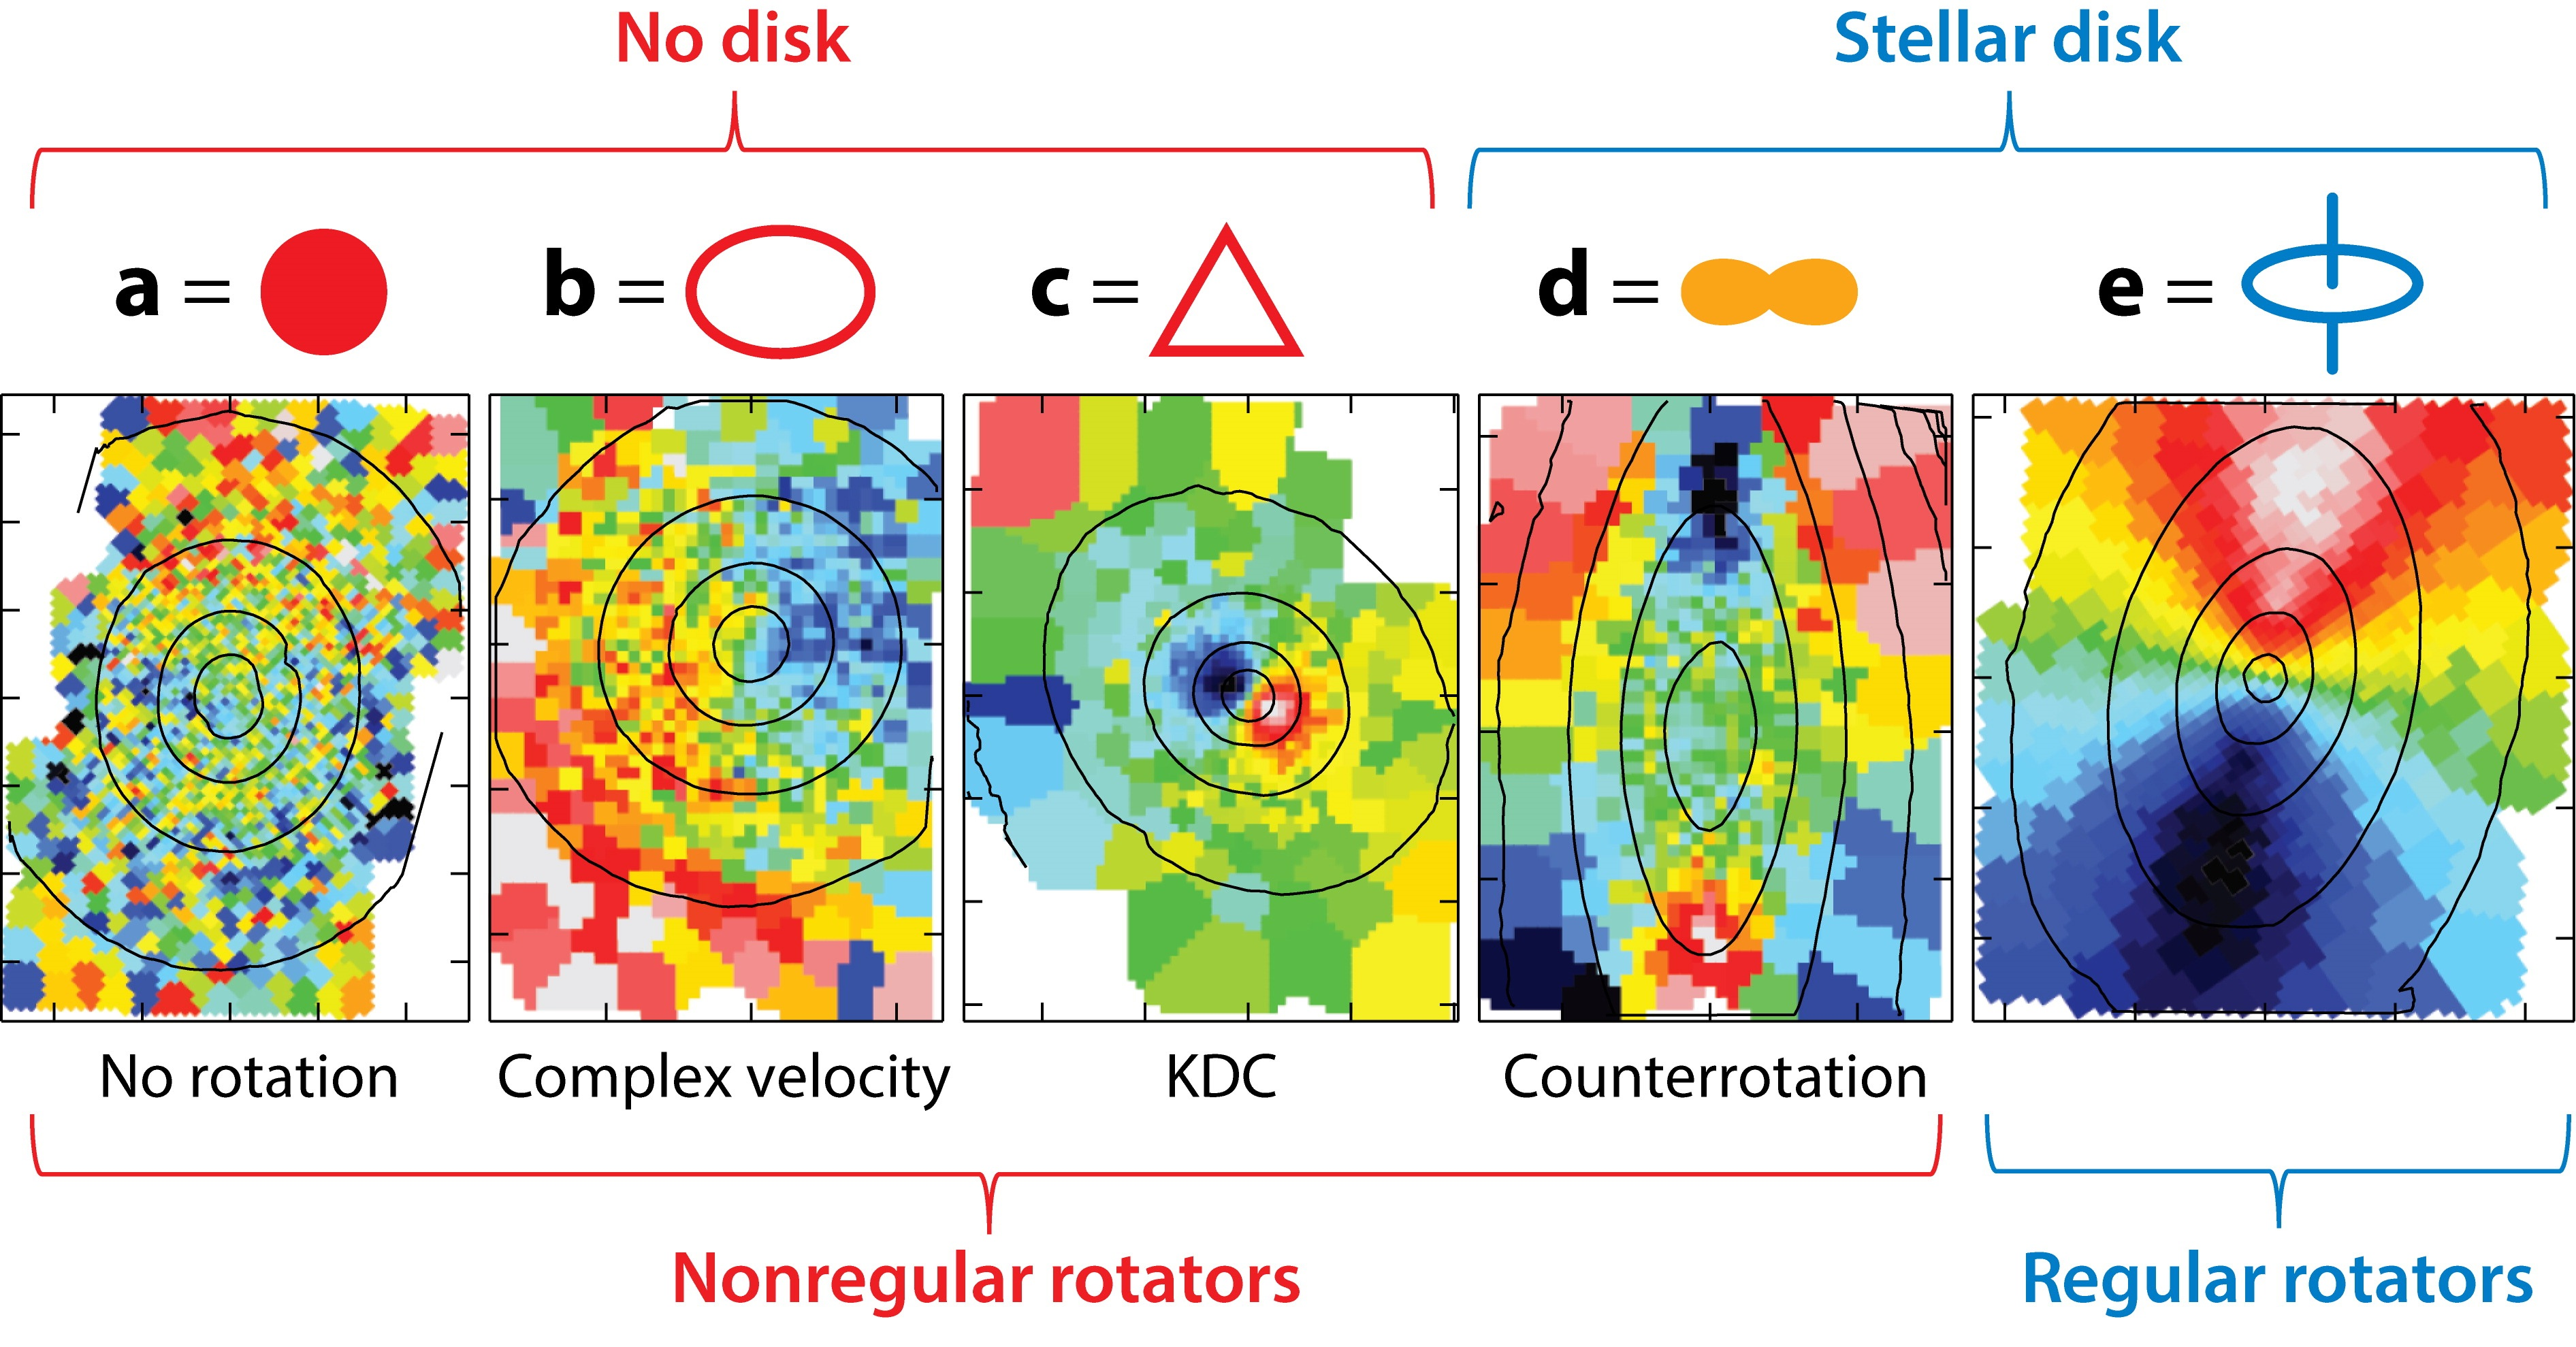
\includegraphics[width=\textwidth]{introduction/substructure.jpeg}
		\caption[Examples of kinematic substructure classifications]{Examples of kinematic substructure classifications of Atlas$^\text{3D}$ (see Table \ref{tab:KinGroups}). Figure courtesy of \citet{Cappellari2016}.}
		\label{fig:EgSubstructure}
	\end{figure}

	Reader wanting more details should consult the excellent review of IFS studies of ETGs: \citet{Cappellari2016}. 


\section{Active Galactic Nuclei}
	\label{sec:AGN}
	The three main issues that astronomers studying AGN focus on are:
	\begin{enumerate}
		\item the origin of the ISM accreted onto the black hole;
		\item the process by which the ISM is accreted; and
		\item any process by which the AGN might affect the host galaxy (feedback).
	\end{enumerate}
	As mentioned previously, the final point has been invoked (and indeed seems to be required) in numerous semi-analytic models and numerical simulations to successfully reproduce the known properties of massive galaxies \citep[e.g.][etc.]{DiMatteo2005, Bower2006, Springel2005}. This mostly involves stopping the bulk of the gas from cooling, such that it can no longer collapse to form stars, with the side-effect that it also self-regulates accretion onto the black hole.

	As previously stated, AGN feedback can be broadly separated into two modes: radiative- and jet-dominated. The former is thought to be the powerful engine that initially rapidly shuts off star formation \citep[e.g.][]{Thomas2005, Thomas2010}, either by removing the cold gas from the galaxy entirely, heating it such that it joins the hot X-ray gas often present in massive galaxies \citep[e.g.][]{OSullivan2001}, or rendering it unusable for star formation (such as by stabilising it against collapse; e.g. \citealt{Martig2009}). After a single radiative-mode episode, the AGN is thought to subside to become jet dominated, repeatedly reheating the surrounding ISM to counter any cooling that might allow the cold gas reservoir to replenish (and subsequently form stars). 

	This section will first look at the different AGN global parameters that can be measured. After this, the two different feedback modes (radiative and jet) will be explored.

	\subsection{AGN Parameters}
		\label{subsec:AGNparams}

		\subsubsection{Bolometric Luminosity}
			Perhaps the most basic property of any AGN is its total (bolometric) luminosity. Given the non-spherically symmetric nature of the unified model of AGN, estimating the bolometric luminosity can be a non-trivial task, particularly for obscured (Type 2) AGN. 

		\subsubsection{Black Hole Mass}
			While black holes are not exclusive to AGN, the black hole mass is a parameter useful to understand them, and it is required to calculate the Eddington limit (see Section \ref{subsubsec:Eddington}). Thanks to scaling relations, estimating the black hole mass, $M_\text{BH}$, is relatively simple. In this work we use the black hole mass--galaxy stellar velocity dispersion relation ($M_\text{BH}$--$\sigma_\ast$) of \citet{McConnell2013}:
			\begin{align}
				\log\left(\frac{M_\text{BH}}{\mathrm{M_\odot}}\right) = & \, (8.32 \pm 0.05) + (5.64 \pm 0.32) \log\left(\frac{\sigma_\ast}{200 \, \mathrm{km \, s^{-1}}}\right) \, ,\\
				\intertext{where $\sigma_\ast$ is the luminosity-weighted stellar velocity dispersion within one effective radius, defined as} 
				\sigma_\ast^2 \equiv & \, \frac{\int_0^{R_\mathrm{e}} \left[\sigma^2(r) + v^2(r)\right] I(r) \, \mathrm{d}r}{\int_0^{R_\mathrm{e}} I(r) \, \mathrm{d}r} \, ,
			\end{align}
			where $I(r)$, $v(r)$ and $\sigma(r)$ are the stellar surface brightness, mean velocity and velocity dispersion at a projected radius $r$.


		\subsubsection{Eddington Ratio}
			\label{subsubsec:Eddington}
			The Eddington ratio, $L/L_\text{Edd}$, is the ratio of the bolometric luminosity, $L$, to the maximum luminosity the AGN can achieve while remaining in hydrostatic equilibrium (the Eddington limit $L_\text{Edd}$). The Eddington limit for pure ionised hydrogen is
			\begin{align}
				L_\text{Edd} = & \,\frac{4 \pi G m_\mathrm{p} c}{\sigma_\mathrm{T}} M_\text{BH} \, ,
				\label{eq:eddingtonLimit} \\
				\intertext{where $G$ is Newton's gravitational constant, $c$ is the speed of light, $m_\mathrm{p}$ is is the mass of proton and $\sigma_\mathrm{T}$ is the Thomson scattering cross-section for an electron on a proton. This is evaluated to}
				\frac{L_\text{Edd}}{L_\odot} = & \, 3.3 \times 10^4 \, \frac{M_\text{BH}}{\mathrm{M_\odot}} \, .
			\end{align}
			

	\subsection{Radiative Mode}
		\label{subsec:Radiative}
		Radiative mode AGN (also called quasar mode in the literature) are thought to be black holes that are actively growing as matter falls directly on to the event horizon. In this case, the energy expelled as radiation exceeds that expelled by any jet that may be present (most of the energy of a jet is kinetic): radiative mode AGN are typically radiatively efficient, with Eddington ratios of 1-100\%. In order to achieve this level of radiative efficiency the accretion discs must be geometrically thin as thick discs tend to trap radiation, carrying it back inwards with the accreting material. 

		\subsubsection{Fueling}
			\label{subsubsec:RadiativeFueling}
			The theories for the fueling of radiative-mode AGN broadly fall into two categories: external (e.g. mergers or strong tidal interactions) and secular driven. \citet{Heckman2014} argue for of the secular processes and suggest that counter claims have incorrectly handled systematics, though they acknowledge the rare cases of completely bulgeless AGN hosting galaxies such as in \citet{Filippenko1993}, \citet{Satyapal2009} and \citet{Simmons2013} do remain a mystery. 

			One of the main methods to identify mergers or strong interactions in AGN is measuring the lopsidedness, parametrised by the dimensionless quantity $A_1^i$, host galaxies. As detailed in \citet{Reichard2008}, $A_1^i$ is the radially averaged amplitude of the $m=1$ azimuthal Fourier mode between $R_\mathrm{50}$ and $R_\mathrm{90}$, the radii in SDSS $i$-band images enclosing 50\% and 90\% of the total light from the galaxy, normalised to the average surface brightness of the galaxy. They show that while there is a trend for more rapidly growing black holes to be hosted by galaxies with higher average lopsidednesses, but when matched by star-formation history, the AGN hosts showed no excess in lopsidedness. They went on to show that lopsidedness is more strongly correlated with central star formation: it has long been known that interactions drive both lopsidedness and starbursts \citep[e.g.][]{Larson1978}. The stronger dependence of accretion rate on to the black hole on star formation than lopsidedness of the host galaxy is demonstrated in Fig.\,\ref{fig:anisotropy}. This uses the strength of the discontinuity at 4000\,\AA, measured with the dimensionless parameter $D_\mathrm{4000}$, as a proxy for stellar age as young stars produce almost no absorption blue-wards of 4000\,\AA. The quantity, $D_\mathrm{4000}$, is defined as the ratio of the average flux density in the 3750--3950\,\AA\ and 4050--4250\,\AA\ bandpasses. Fig.\,\ref{fig:anisotropy} shows the [\ion{O}{iii}] emission line luminosity (normalised by the black hole mass) is better correlated with the age of the central stellar population than with the lopsidedness of the galaxy. \citet{Heckman2014} interpret this result as ``implying that the fueling of the [AGN] is enhanced by the presence of circumnuclear star formation (and its associated cold gas), but this [AGN] fueling process does not depend upon the way in which this central star formation arises."

			\begin{figure}
				\centering
				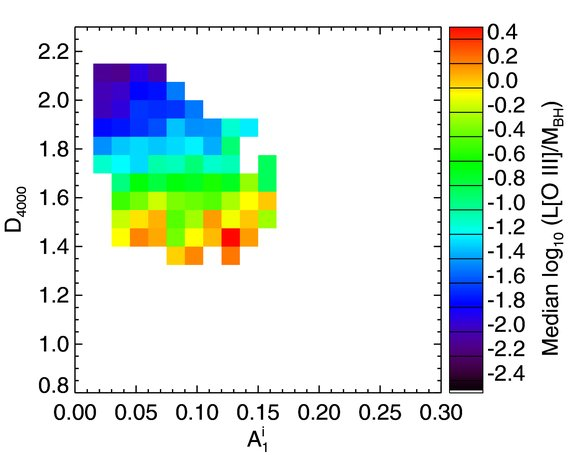
\includegraphics[width=0.6\textwidth]{introduction/age_anisotropy.jpg}
				\caption[The dependence of AGN on age and anisotropies]{AGN strength verses stellar population age and galaxy lopsidedness for SDSS galaxies with redshift $z<0.06$. The AGN strength, quantified by the median luminosity of the [\ion{O}{iii}] emission line normalised by the black hole mass (colour scale) is more strongly dependent on the age of the central stellar population (using $D_\mathrm{4000}$ as a proxy) than on the lopsidedness parameter $A_1^i$. Figure courtesy of \citet{Reichard2009}}
				\label{fig:anisotropy}
			\end{figure}

			Instead, it is thought that secular processes that support inward radial transport of gas are required. These all involve some non-axisymmetric perturbation to the gravitational potential of the galaxy, such as a bar, oval distortion and/or spiral arms \citep[e.g.][]{Kormendy2004, Athanassoula2008, Sellwood2014}. These processes also cause the formation of a so-called pseudobulge, that like a classical bulge is a central region of enhanced surface brightness compared to the extrapolation of the outer (exponential) disc, but unlike a classical bulge is itself disc dominated (i.e. dynamically Col.\,) and often contains significant star formation \citep[e.g.][]{Gadotti2009}. \citet{Kormendy2013a} showed that the transition from classical bulges to pseudobulges occurs at a black hole mass of $M_\text{BH} \sim 10^7\,\mathrm{M_\odot}$, corresponding to a bulge stellar velocity dispersion of $\sigma \approx 150 \, \mathrm{km \, s^{-1}}$, which is also where the bulk of local black hole growth is occurring \citep[e.g.][]{Heckman2004, Kauffmann2009}. 

			Finally it is worth noting that bars do not seem to enhance nuclear activity, except that like AGN they are more common in more massive (and redder) galaxies. Once colour and mass are fixed, there is no excess of AGN in strongly-barred galaxies \citep[e.g.][]{Lee2012, Cisternas2013}. This suggests that, while the AGN clearly requires some process to move gas radially inwards, the strength of the AGN is not coupled to the strength of a large-scale bar. 


		\subsubsection{Feedback}
			\label{subsubsec:RadiativeFeedback}
			It is thought radiative mode AGN can also drive powerful interstellar winds, capable of terminating star formation and thus moving a galaxy from the blue cloud to the red sequence. Indeed such strong winds have been observed with velocities in excess of 1000 km s$^{-1}$ \citep{Fischer2010, Feruglio2010, Rupke2011} and \citet{Page2012} showed that (high-level) star formation is present in AGN with X-ray luminosities less than $10^{44} \, \mathrm{erg \, s^{-1}}$, but not above this. Having said that, many radiative-mode AGN actually have circumnuclear star-formation enhancement, presumably due to some of the accreted material being turned into stars \citep[e.g.][]{Santini2012}. 

			The feedback process must also be responsible for maintaining the $M_\text{BH}$--$\sigma_\ast$ relation. If we assume that radiation pressure from an Eddington luminosity AGN sweeps up a gas mass $M_\text{gas} = f M_\text{gal}$ (i.e. $f$ is the fraction of the mass of the galaxy, $M_\text{gal}$, that is in the AGN wind), then the force from this radiation pressure, $F_\text{out}$, should match the force due inward gravitational pressure, $F_\text{in}$.
			\begin{align}
				\frac{L_\text{edd}}{c} = F_\mathrm{out} = & \, F_\text{in} = \frac{G M_\text{gal} M_\text{gas}}{r^2} \, , \\
				\intertext{substituting $M_\text{gas} = f M_\text{gal}$, the dynamical mass $M_\text{gal} = \frac{2\sigma_\ast^2 r}{G}$ and Equation \ref{eq:eddingtonLimit}, and rearranging yields}
				M_\text{BH} = & \frac{f \sigma_\ast^4 \sigma_\mathrm{T}}{\pi G^2 m_\mathrm{p}} \, .
				\label{eq:MSigma}
			\end{align}
			This is known as a momentum driven wind \citep[e.g.][]{Fabian1999} and is consistent with some measurements of the $M_\text{BH}$--$\sigma_\ast$ relation, such as that of \citet{Gultekin2009}.
			Another theoretical model for the driving of AGN winds is that they are thermally driven \citep{Silk1998}. This predicts a power-law with an index of $\approx 5$ i.e. $\frac{\mathrm{d} \log M_\mathrm{BH}}{\mathrm{d}\log \sigma_\ast} \approx 5$ (as opposed to $\approx 4$ in momentum-driven winds as in Eq. \ref{eq:MSigma}), which is more consistent with more recent measurements of the $M_\mathrm{BH}$--$\sigma_\ast$ relation \citep[e.g.][]{McConnell2013}. 
			Whatever the process that couples the AGN to the winds, the general consensus in the literature is that these winds are responsible for removing or destroying much of the cold gas of the host galaxy, effectively shutting off star formation via the starving of the galaxy of fuel. 
		\subsubsection{Radiative-mode Radio Galaxies}
			\label{subsubsec:RadiativeRadio}
			As stated above, the most powerful RGs are radiative-mode AGN. This is in spite of the fact that RGs are markers for jets (and the radio power is directly correlated with the jet strength). This implies that at these energies, the processes that drive the radiation from the accretion discs must also be more sensitive to the environmental conditions than the processes that drive the jets. RGs are more common at high redshifts, $1.5 \lesssim z \lesssim 3$, which is sometimes called the quasar era \citep{Miley2008}. \citet{Gopal-Krishna2001} suggested that the massive radio lobes from these objects may have been responsible for permeating much of the material that led to the peak of star formation at $z \approx 1.5$. Indeed strong outflows, assumed to be driven by the mechanical energy of the jets, are observed at theses epochs \citep[e.g.][]{Nesvadba2008, Maiolino2012}.
			The broad consensus in the literature is that RGs require a major wet merger to form \citep[e.g.][]{Malin1983, Quillen1992, Lim2000}. Our sample of RGs described in Section \ref{sec:Sample} does not contain any of these extreme galaxies.
	\subsection{Jet Mode}
		\label{subsec:Jet}
		In jet-mode (also called radio- or maintenance-mode in the literature) AGN, the dominant form of emitted energy away from the black hole is the kinetic (i.e. mechanical) energy of the material that makes up the jet. Jet-mode AGN can be directly observed `feeding back' to their host galaxies, as jets often terminate at shocks (hot spots) that make up the walls of cavities observed in the hot (X-ray) haloes of the host galaxies.

		Jet-mode AGN tend to be radiatively inefficient, with Eddington ratios $<$ 1\%. This implies that the innermost regions of the accretion discs must be geometrically thick, with inflow times much less than the radiative cooling timescales. The resulting inflows are known as advection-dominated accretion flows (ADAF; \citealt{Narayan1994}). Such systems are capable of launching jets. It is possible that there is a thin disc beyond the thick disc (further from the black hole), but it must be truncated by the thick disc \cite[e.g.][]{Abramowicz2002, Sadler2014}. Much of this is very difficult to resolve observationally, as the spatial scale is $< 100$ Schwarzschild radii, and many of the models remain degenerate \citep[e.g.][]{Quataert1999}. 

		\subsubsection{Fueling}
			\label{subsubsec:JetFueling}
			There is still much speculation about the nature of the fuel (and its origin) in jet-mode AGN, though a consensus seems to building in favour of an internal origin. Many people advocate hot gas as being the ultimate original fuel \citep[e.g.][]{Allen2006}. \citet{Hardcastle2007a} suggest that it could be directly accreted through Bondi accretion \citep{Bondi1952}, a simple model where gas is accreted in a spherically-symmetric manner directly from the hot phase onto the black hole. Others invoke a cooling mechanism to allow the X-ray gas to condense into molecular (i.e. cold) gas before accretion. Yet others point to a higher higher detection rate of dust and molecular gas in RGs compared to the general population \citep[e.g.][]{Lim2000, DeRuiter2002,Lim2003, VerdoesKleijn2005}, suggesting that cold gas from either internal reservoirs or externally-accreted may be the fuel. \citet{DeRuiter2002} showed that, when dust is present, its mass is correlated with the radio power and there seems to be a bias towards dust lanes orientated orthogonally to radio jets \citep{VerdoesKleijn2005}.

			Beyond this, the source of the energy for powering the jet is still unclear. Energy may be extracted from the black hole via the \citet{Blandford1977} mechanism or variations thereof \citep[e.g.][]{Koide2002}, or from the accretion disc as discussed by \citet{Blandford1982} and others \citep[e.g.][]{Hujeirat2003}. 

		\subsubsection{Feedback}
			\label{subsubsec:JetFeedback}
			It is thought that the duty cycle of a jet is very short; the jet is turned on for very short periods of time before turning off for extended periods. 

			An obvious feedback mode is seen in the haloes of hot X-ray gas around galaxies, where radio jets terminate. The kinetic impacts of the jets create cavities or bubbles in the hot gas (first conceptualised by \citealt{Gull1973}). In cluster environments, these are buoyant and can separate, rising through the intra-cluster medium \citep[e.g.][]{Churazov2000, Churazov2001, McNamara2000}. However, the bubbles are intrinsically anisotropic, while star formation must be suppressed on a global scale. They also exhibit steep abundance gradients, showing that there is little mixing that could disperse energy via convection. Instead, from observations of the very brightest X-ray clusters such as Perseus \citep{Fabian2003, Fabian2006}, Virgo \citep{Forman2007}, Centaurus \citep{Sanders2008}, Abell 2052 \citep{Blanton2011} and simulations \citep[e.g.][]{Ruszkowski2004, Sijacki2006}, it appears that sound waves in the ISM are generated by the repetitive blowing of bubbles. The energy of the waves is likely sufficient to offset that lost by the gas via normal cooling mechanisms \citep{Fabian2003}. The low amplitude of these waves means that they are not detectable in all but the closest clusters (more distant clusters would require in excess of 10 days of continuous \textit{Chandra} observations; \citealt{Graham2008}).

			Even when the jets are turned off or only very weak, the galaxies may still contain low ionisation nuclear emission-line regions (LINERs). It is worth noting that while the most powerful LINERs are likely to be low-luminosity AGN, many (indeed most SDSS-classified LINERs) are not; they belong to a recently-defined category known as LIERs i.e. the emission-line region is not nuclear (LINERs but without the 'N'; e.g. \citealt{Sarzi2005, Sarzi2010, Singh2013, Belfiore2016a}). Such emission is mostly attributed to ionisation from radiation from post-asymptotic giant branch (pAGB) stars. \citet{Capetti2011} suggested using an equivalent width of the [\ion{O}{iii}] emission line of $EW_\text{[\ion{O}{iii}]} = 1$\,\AA\ as a threshold for LIERs; galaxies with greater equivalent widths are likely low-luminosity AGN.

		\subsubsection{Jet-mode Radio Galaxies}
			\label{subsubsec:JetRadio}
			As stated above, most radio emission from RGs results from synchrotron emission from the relativistic plasma within the jets, moving around the magnetic fields tangled in the jets. This means that all such RGs can be considered a jet detection (ignoring the very low radio-luminosity galaxies resulting from high levels of circumnuclear star formation). RGs are always jet-mode AGN, except at the highest radio luminosities where the bright radio jets are dominated (in terms of energy output) by the brighter still accretion disc. These are radiative-mode AGN (see Section \ref{subsubsec:RadiativeRadio}).

			All radio-selected AGN are massive, with very old stellar populations and high concentration indices \citep[e.g.][]{Best2005}. \citet{Best2005} also found that the fraction of galaxies with detectable radio emission is related to the galaxies' stellar and black hole masses by power laws with indices of 2.5 and 1.6, respectively.

	Reader wanting more details on the co-evolution of black holes and host galaxies, and the role of AGN, should consult the excellent reviews by \citet{Fabian2012} and \citet{Heckman2014}. 

\section{Southern Sample}
	\label{sec:Sample}

	\begin{table}
		\centering
		\caption{Key sample selection criteria.}
		\label{tab:selection}
		\begin{tabular}{l c}
			\hline
			\hline
			Declination				& $-17\degree < \delta < -40\degree$ \\
			2.7\,GHz flux density 		& $S_\text{2.7GHz} \ge 0.25 \, \text{Jy} $ \\
			$V$-band apparent magnitude 	& $m_V \le 17.0 $ \\
			Redshift 					& $z < 0.03$ \\			
			\hline
			\hline
		\end{tabular}
	\end{table}

	To study RGs in better detail, a sample of 11 galaxies in the southern hemisphere was constructed by \citet{Prandoni2010}. This sample is similar to the B2 sample of northern hemisphere RGs \citep{Prandoni2007}.

	The Parkes 2.7 GHz survey \citep{Ekers1989} was used as a parent sample, as it contains radio sources (down to a flux density limit of 250\,mJy at 2.7\,GHz) with an optical counterpart (with an $V$-band apparent magnitude of $m_V \le 17.0$). Host galaxies with a redshift greater than 0.03 were discarded. The selection criteria are summarised in Table \ref{tab:selection}. It is worth noting that both the radio and optical limits are apparent measurements, and as such this is not a volume-limited sample.

	\begin{table}
		\centering
	\begin{threeparttable}
		\caption{Key sample characteristics of the Southern Sample galaxies.}
		\label{tab:sample}
		\begin{tabular}{l l r r r l}
			\hline
			\hline
			Host galaxy	& Radio source 	& Redshift	& $S_\text{1.4\,GHz}$	& $m_K$ & Dust morphology\\
						& (PKS) 		& 			& (mJy) 			& (mag)	&\\
			\hline 
			ESO 443-G024 & 1258-321 	& 0.01703	& $1387 \pm 45$		& 8.51 & no dust\tnote{a}	\\ 
			IC 1459 	& 2254-367 		& 0.00565 	& $1280 \pm 45$		& 6.81 & dust lane\tnote{b}	\\
			IC 1531 	& 0007-325 		& 0.02553 	& $388 \pm 12$		& 9.55 & --					\\
			IC 4296		& 1333-\leavevmode\phantom{0}33 		& 0.01248 	& $1342 \pm 41$		& 7.50 & edge-on disc\tnote{b} \\
			NGC 612 	& 0131-\leavevmode\phantom{0}36 		& 0.02954 	& $585 \pm 18$		& 9.58 & dust lane\tnote{c}	\\
			NGC 1316 	& 0320-\leavevmode\phantom{0}37 & 0.00591 	& $255 \pm 10$		& 5.59 & dust patches\tnote{b} \\
			NGC 1399 	& 0336-\leavevmode\phantom{0}35 & 0.00472 	& $209 \pm \leavevmode\phantom{0}7$	& 6.31 & no dust\tnote{b}	\\
			NGC 3100 	& 0958-314 		& 0.00879 	& $530 \pm 16$		& 8.08 & dust lane\tnote{d}	\\
			NGC 3557 	& 1107-372 		& 0.01016 	& $484 \pm 16$		& 7.203 & face-on disc\tnote{b}\\
			NGC 7075 	& 2128-388 		& 0.01819 	& $837 \pm 28$		& 9.56 & --					\\
			--			& 0718-\leavevmode\phantom{0}34 		& 0.02897 	& $1119 \pm 41$		& 9.97 & dust patches\tnote{e} \\
			\hline
			\hline
		\end{tabular}
		\begin{tablenotes}
		\footnotesize
		\note Col.\,1: host galaxy name. Col.\,2: radio source name from Parkes Southern Radio Source Catalogue. Col.\,3: redshift. Col.\,4: National Radio Astronomy Observatory (NRAO) Very Large Array (VLA) Sky Survey (NVSS) 1.4 GHz flux density \citep{Condon1998}. Col.\,5: Two Micron All Sky Survey (2MASS) $K$-band apparent magnitude (with errors of $\pm 0.025$ mag; \citealt{Skrutskie2006}). Col.\,6: dust morphologies from (a) \citet{Govoni2000}, (b) \citet{Lauer2005}, (c) \citet{Bettoni2001}, (d) \citet{Sandage1979}, (e) \citet{Colbert2001}. 
		\item We hereafter refer to the last galaxy by its PKS name only.
		\end{tablenotes}
	\end{threeparttable}
	\end{table}

	These criteria lead to a sample of 11 galaxies hereafter referred to as the Southern Sample. The key observed characteristics are summarised in Table \ref{tab:sample}, while the derived characteristics are listed in Table \ref{tab:sampleDerived}. All galaxies have a FR I radio morphology according to the \citet{Fanaroff1974} scheme; the bulk of the radio emission is centrally-concentrated, as opposed to the FR II morphology where the brightest points are at the ends of the radio lobes. 
	
	The sample was initially observed with the Atacama Pathfinder Experiment (APEX), with detections claimed for the \ce{^{12}CO(2-1)} transition for all galaxies. Some galaxies had extremely large line widths (up to a full-width half-maximum of $904 \, \mathrm{km \, s^{-1}}$ for IC 4296), but most showed a flat or double-horn spectrum indicative of ordered rotation \citep{Prandoni2012}.

	\begin{table}
		\centering
	\begin{threeparttable}[b]
		\caption{Derived characteristics of the Southern Sample galaxies.}
		\label{tab:sampleDerived}
		\begin{tabular*}{\textwidth}{@{\extracolsep{\fill}}l l l l}

			\hline
			\hline
			Host galaxy	& $M_K$ & $\log P_\text{1.4\,GHz}$ & Spectral index 	\\
						& (mag)	& ([W Hz$^{-1}$])		& ([Jy][GHz]$^{-1}$) 	\\
			\hline 
			ESO 443-G024 & -25.86 & 24.0 				& $-0.56 \pm 0.08$	\\
			IC 1459 	& -25.27 & 23.0 				& $\leavevmode\phantom{-}0.25 \pm 0.06$\tnote{a} 	\\
			IC 1531 	& -25.70 & 23.9 				& $-0.33 \pm 0.03$ 	\\
			IC 4296		& -26.18 & 25.4 				& $-1.52 \pm 0.27$ 	\\
			NGC 612 	& -26.01 & 25.0 				& $-1.05 \pm 0.24$ 	\\
			NGC 1316 	& -26.44 & 22.4 				& $-4.7\leavevmode\phantom{0} \pm 2.1\leavevmode\phantom{0}$ 	\\
			NGC 1399 	& -25.25 & 22.5 				& $-0.65 \pm 0.66$ 	\\
			NGC 3100 	& -24.85 & 23.0 				& $-0.40 \pm 0.03$ 	\\
			NGC 3557 	& -26.08 & 23.3 				& $-0.72 \pm 0.13$ 	\\
			NGC 7075 	& -24.98 & 23.9 				& $-0.90 \pm 0.06$ 	\\
			PKS 0718-34 & -25.59 & 24.6 				& $-0.63 \pm 0.06$ 	\\
			\hline
			\hline
			% Also need to correct P_1.4 values are I have changed the S_1.4 values to NVSS in tab:sample
		\end{tabular*}
		\begin{tablenotes}
		\footnotesize
		\note Col.\,1: galaxy name. Col.\,2: $K$-band absolute magnitude. Col.\,3: 1.4 GHz radio power. Col.\,4: radio spectral index (from a straight line fitted to the logarithm of all data points below 10 GHz taken from the Photometric Points tool in the Strasbourg astronomical Data Center (CDS) Portal \citealt{Wenger2000}).
		\item [a] IC 1459 shows a turn over in its spectral energy distribution at $\approx 1 \, \text{GHz}$ (see Fig.\,\ref{fig:ic1459radio}) i.e. it is a gigahertz-peaked spectrum (GPS) galaxy. This means the spectral index is very sensitive to the frequency range over which is measured.
		\end{tablenotes}
	\end{threeparttable}
	\end{table}
